% Choose the language of your thesis passing 'french' or 'english' as
% \documentclass option.
% Note1: The 'page de garde' will always be written in French.
% Note2: You will have an error if you change the language of the document and
%        compile it without cleaning the auxiliary files. Compiling it again
%        should solve the problem.
\documentclass[french,a4paper,11pt,twoside]{StyleThese}
\newcommand{\included}{}

\include{formatAndDefs}
\usepackage{pifont}
\usepackage{subcaption}

\usepackage[acronym,nogroupskip,nonumberlist]{glossaries}  % pour gérer les acronymes aussi

\renewcommand*{\glsnamefont}[1]{\textbf{#1}}

% Intro
\newacronym{pepr}{PEPR}{Programmes et Equipements Priotaires de Recherche}
\newacronym{gnn}{GNN}{Réseaux de Neurones sur Graphes}
\newacronym{3gpp}{3GPP}{3rd Generation Partnership Project}
\newacronym{ran}{RAN}{Réseau d'Accès Radio}

% --------- Chapitre 1 
\newacronym{nf}{NF}{Fonction Réseau}
\newacronym{nfv}{NFV}{Virtualisation des Fonctions Réseaux}
\newacronym{cn}{CN}{Cœur de Réseau}
\newacronym{dn}{DN}{Réseau de Donnée}
\newacronym{ids}{IDS}{Système de Détection d'Intrusion}
\newacronym{ue}{UE}{Equipment utilisateurs}
\newacronym{seid}{SEID}{Identifiant de Session}
\newacronym{teid}{TEID}{Identifiant de Tunnel}
\newacronym{sm}{SM}{Gestion de Session}
\newacronym{an}{AN}{Réseau d'Accès}
\newacronym{gnb}{gNB}{Next Generation NodeB}
\newacronym{far}{FAR}{Forwarding Action Rule}
\newacronym{mitm}{MITM}{Man-in-the-middle}

% Network Functions spécifiques à la 5G
\newacronym{nrf}{NRF}{Network Repository Function}
\newacronym{upf}{UPF}{User Plane Function}
\newacronym{smf}{SMF}{Session Management Function}
\newacronym{amf}{AMF}{Access and Mobility Management Function}
\newacronym{ausf}{AUSF}{Authentication Server Function}
\newacronym{udm}{UDM}{Unified Data Management}
\newacronym{udr}{UDR}{Unified Data Repository}
\newacronym{pcf}{PCF}{Policy Control Function}
\newacronym{scp}{SCP}{Service Communication Proxy}

% Protocoles 5G
\newacronym{pfcp}{PFCP}{Packet Forwarding Control Protocol}
\newacronym{nas}{NAS}{Non-Access Stratum}
\newacronym{ngap}{NGAP}{Next Generation Application Protocol}
\newacronym{gtp}{GTP}{GPRS Tunneling Protocol - User Data}
\newacronym{http2}{HTTP/2}{Hypertext Transfer Protocol/2}

% Autres
\newacronym{api}{API}{Application Programming Interface}
\newacronym{tls}{TLS}{Transport Layer Security}


\newacronym{sbi}{SBI}{Service-Based Interfaces}
\newacronym{oai}{OAI}{Open Air Interface}
\newacronym{ddos}{DDoS}{Déni de Service Distribué}
\newacronym{sdr}{SDR}{Radio Définie par Logiciel}

% --------- Chapitre 2
\newacronym{smc}{SMC}{Security Mode Command}
\newacronym{suci}{SUCI}{Subscriber Concealed Identifier}


% --------- Chapitre 3
\newacronym{svm}{SVM}{Machines à Vecteurs de Support}
\newacronym{cnn}{CNN}{Réseaux de Neurones Convolutionnels}
\newacronym{imsi}{IMSI}{Identifiants Utilisateurs}
\newacronym{rnn}{RNN}{Réseau de Neurones Récurrent}
\newacronym{gru}{GRU}{Gated Reccurent Unit}
\newacronym{fl}{FL}{Federated Learning}
\newacronym{nlp}{NLP}{Traitement Automatique du Langage Naturel}
\newacronym{gcn}{GCN}{Graph Convolutional Networks}
\newacronym{gin}{GIN}{Graph Isomorphism Networks}
\newacronym{gat}{GAT}{Graph Attention Networks}
\newacronym{dtgn}{DTGN}{Réseaux de Graphes à Temps Discret}
\newacronym{pca}{PCA}{Analyse en Composantes Principales}
\newacronym{cbow}{CBOW}{Continuous Bag of Words}
\newacronym{glove}{GloVe}{Global Vectors for Word Representation}

% --------- Chapitre 4
\newacronym{mpn}{MPN}{Réseaux Privés Mobiles}
% \newacronym{}{}{}
% \newacronym{}{}{}
% \newacronym{}{}{}
% \newacronym{}{}{}


\makeglossaries  % commande pour générer le glossaire


\sloppy
\begin{document}

\include{page_de_garde}

\makeflyleaf

 \cleardoublepage

\dominitoc

\pagenumbering{roman}

 \cleardoublepage

% Here you can see an example of how to create text conditioned by the language
% variable. The \iftoggle command:
%
%   \iftoggle{ThesisInEnglish}{%
%   <your-text-in-english>
%   }{%
%   <your-text-in-french>
%   }
%
% will compile only one of the two blocks, depending on the variable you set at
% the beginning of this document. Language selection is managed this way in the
% formatAndDefs.tex file. You too can create sections of your thesis that is
% language dependend this way, although you probably won't need it. Another use
% of \iftoggle can be found at the end of this file.
\iftoggle{ThesisInEnglish}{%
\section*{Acknowledgments}
}{%
\section*{Remerciements}
}


"La thèse c'est un marathon", en tout cas c'est ce qu'on m'a dit lors de mes premiers jours. Je n'ai jamais couru de marathon (malgré le forcing de mes collègues adorés) mais j'imagine un trajet balisé où le seul problème c'est de tenir la distance. Moi la thèse, je la vois plutôt comme un marathon, oui, mais avec les yeux bandés, sur un trajet qui ressemble à un plat de spaghetti, et avec une petite voix qui te hurle dans les oreilles que tu n'es pas légitime. 

Ça sonne pas terrible dit comme ça mais, heureusement, une thèse ça se fait pas tout à fait seul. Au cours de mon parcours j'ai eu la chance de rencontrer des personnes formidables qui ont donné du sens à tout ce bazar et m'ont permis de tenir la distance sans (trop) m'égarer. Ça à avant tout été une aventure humaine et je pense que c'est sur plan-là que j'ai le plus évolué. Merci à toutes celles et ceux que j'ai pu croiser sur mon chemin, que ce soit dans le cadre de mes travaux ou en dehors. 

% Philippe 
Philippe. Pendant mes premiers jours au labo, tu as rencontré un jeune ingénieur un peu perdu, timide et pas très sûr de lui. Ton objectif était de me "transformer en chercheur", que je développe mon assurance et que je puisse te tenir tête. Je pense que tu as réussi. Ces trois ans n'ont pas toujours été faciles. Il y a eu des gros moments de doute et de découragement. Dans ces moments-là, je rentrais dans ton bureau, sans vraiment avoir quelque chose de particulier à dire. À chaque fois, tu sentais ma détresse et tu trouvais les bons mots pour me rebooster. Merci beaucoup, Philippe, pour ton soutien, tes conseils et ton temps. Je suis très heureux d'avoir fait cette aventure avec toi. 

% Jury
Je tiens aussi à remercier Michaël Hauspie, Xavier Lagrange, Nathalie Mitton, Eric Totel et Yassine Hadjadj-Aoul pour avoir accepté de faire partie de mon jury, pour leurs retours constructifs sur le manuscrit et l'intérêt général qu'ils ont porté à mes travaux. Un remerciement particulier à Yassine pour le temps que tu m'as accordé lors de nos discussions sur les GNN. Merci aussi à Eric et Vincent qui m'ont suivi depuis le début de ma thèse à travers les rendez-vous CSI.

% HiSec
Une pensée aussi aux collègues du projet HiSec, avec qui j'ai pu échanger tout au long de ma thèse. Je ne pourrai pas citer tout le monde mais merci notamment à Guillaume, Gregory et Issam avec qui j'ai eu la chance de collaborer plus étroitement. Le papier que nous avons réalisé ensemble a été un vrai bol d'air frais dans ma thèse et m'a ouvert à de nouvelles perspectives autant sur la recherche en elle-même que sur la façon de mettre en valeur nos résultats. Merci aussi à toutes celles et ceux avec qui j'ai pu collaborer et à qui j'ai pu poser des questions en rapport avec mes travaux : Alexandre, Romain, Florent, Marie-José, Damien, Matthieu\dots Enfin merci à Mariam et Guillhem : vous êtes les deux premiers stagiaires que j'ai eu la chance d'encadrer et je pense que j'aurai difficilement pu mieux tomber. Vous avez tous les deux été très impliqués et motivés, c'était un vrai plaisir de pouvoir échanger avec vous et je vous souhaite de tout mon cœur le meilleur pour la suite.

\newpage

% Collègues
Au début de la thèse, Philippe m'a dit que les doctorants que je rencontrerai deviendraient sans doute des amis proches, bien au-delà de la thèse. Effectivement, partager ses galères, ses peines et ses rires avec des gens qui te comprennent, ça rapproche. Vous êtes des êtres humains formidables et j'ai énormément de chance d'avoir pu vivre ce morceau de vie avec vous. Le temps est passé très vite mais je garderai précieusement en moi les souvenirs de ces moments partagés. 
Merci à Stanislas et Matthieu, mes premiers repères, les seuls qui auront réussi à me faire me lever à 5h pour faire du sport. 
Merci à Zheng et son humour dévastateur pour ces soirées sur LoL jusqu'à des heures impossibles. 
Merci à Minh pour ces innombrables pauses clopes et les subséquentes discussions sur nos expés ratées, sur la vie et sur nos goûts musicaux discutables.   
Merci à Antony, la personne la plus généreuse et bienveillante que j'ai eu la chance de rencontrer. 
Merci à la voiture d'Antony pour tous ces trajets à 3h du matin. 
Merci à Mathis pour ton empathie et toutes ces discussions à cœur ouvert.  
Merci à Zac de m'avoir aidé à remettre énormément de choses en perspective, que ce soit dans ma thèse ou en dehors. 
Merci à Edouard et Cédric de m'avoir montré que c'était OK d'être nul aux jeux vidéos.
Merci à Miguel pour ton extravagance et d'être aussi bon public.
Merci à Florian et Claude pour votre spontanéité et votre enthousiasme. 
Merci à Oumayma pour les petites attentions quand tu remarquais que ça n'allait pas fort. 
Merci à Feras et Kader pour votre sagesse et vos traits d'esprit. 
Merci à Léonard de m'avoir fait confiance dans les moments difficiles. 
Merci à Slim, Pascal et Ahmed pour votre bonne humeur communicative et vos mots encourageants. 
Merci à Gabin, Céline et Clément, mes prédécesseurs, pour m'avoir guidé du début à la fin. 
Merci aussi à tous les autres : Christian, Thouria, Cheickna, Alexandre, Lenny, Jacques\dots

% Amis
Merci aussi bien sûr aux amis de longue date dont le soutien à toujours eu une valeur inestimable. Antoine et Matthieu, ma fine équipe du lundi. Fiora, Lisa et Mariale, toujours là dans les moments difficiles. Paul, mon plus fidèle relecteur. Fabien et Nolan pour leurs conseils avisés. Antonin et Viktor qui arrivent systématiquement à me faire rire. Elea pour sa résilience inspirante. Héloïse pour son énergie et sa gentillesse.

% Famille
Enfin, merci à ma famille. Merci à mes frères et sœurs : Romain, Bastien, Adeline. Merci à mes parents. Vous avez toujours soutenu et encouragé chacunes de mes décisions. Je sais que vous auriez été fiers de moi quel que soit mon parcours mais si je suis allé jusqu'au bout de cette thèse c'était aussi en pensant à vous.

\vspace{2cm}

\begin{figure}[h]
\centering

\includegraphics[width=0.7\linewidth]{figures/chapter0/Merci.png}
\label{fig:merci}
\end{figure}

\cleardoublepage

\section*{Abstract}
Pour répondre à de nouvelles exigences de qualité de service et à l’émergence de nouveaux usages, le paradigme de la 5G marque une rupture majeure avec les architectures réseau traditionnelles. Le cœur de réseau évolue d’un système monolithique, dans lequel chaque fonction réseau est statiquement associée à un équipement matériel dédié, vers une architecture logicielle virtualisée, flexible et dynamique. À l’image des architectures à microservices, les fonctions réseau peuvent désormais être déployées, modifiées ou supprimées à la demande, rapprochant ainsi la 5G des systèmes distribués modernes.

Cette transformation apporte toutefois de nouveaux défis en matière de sécurité. La virtualisation et la distribution des fonctions réseau élargissent la surface d’attaque et favorisent l’émergence de menaces inédites, difficilement détectables à l’aide des approches traditionnelles de volumétrie ou de signature. Dans ce contexte, il devient nécessaire de dépasser les méthodes classiques employées par les systèmes de détection d’intrusion et d’adopter des approches centrées sur le paquet, capables d’analyser simultanément son contenu, son contexte temporel ainsi que son rôle au sein des interactions réseau.

Afin de capturer ces dimensions sémantiques, séquentielles et topologiques, cette thèse propose un nouveau formalisme fondé sur les graphes continus dynamiques. Cette représentation permet de modéliser finement l’évolution des communications réseau et d’exploiter les capacités des \gls{gnn}. Les travaux présentés démontrent que cette approche permet de détecter efficacement des anomalies subtiles tout en offrant un niveau élevé d’interprétabilité, indispensable à leur analyse et à leur compréhension.

\textbf{Mots clés:} Cybersecurité, 5G, Détection d'Anomalie, GNN Dynamique, NLP, Dataset

\newpage

\section*{Abstract}
To address emerging quality-of-service requirements and support new use cases, the 5G paradigm represents a major shift from traditional network architectures. The core network is evolving from a monolithic system, in which each network function is statically tied to dedicated hardware, toward a flexible, software-based, virtualized architecture. Similar to microservice-oriented systems, network functions can now be dynamically deployed, scaled, and removed according to operational needs, bringing 5G architectures closer to modern distributed systems. 

However, this transformation also introduces new security challenges. The virtualization and distribution of network functions expand the attack surface and enable the emergence of novel threats. Some of these attacks can be carried out using only a handful of abnormal packets, making them particularly difficult to detect using traditional intrusion detection approaches based on volumetric features or predefined signatures. As a result, securing next-generation networks requires moving beyond conventional metric-driven methods and adopting packet-level approaches capable of jointly analyzing packet contents, temporal context, and interaction patterns within network communications. 

To capture these semantic, sequential, and relational dimensions, this thesis introduces a novel framework based on Continuous Dynamic Graphs. This representation enables a fine-grained modeling of the evolving structure of network communications while leveraging the expressive power of \gls{gnn}. The proposed approach effectively detects subtle and previously hard-to-identify anomalies while providing a high degree of interpretability, a key requirement for security analysis and operational deployment

\textbf{Keywords:} 5G, Cybersecurity, Anomaly detection, Dynamic GNN, NLP, Dataset


\cleardoublepage

% \section*{Résumé}


\tableofcontents

\printnomenclature
% Use \mtcfixnomenclature below if you have a glossary (added with
% \printnomenclature above) and you're see a shift in the mini-table of
% contents at the begining of each chapter (example: no mini-toc in chapter 1;
% mini-toc of chapter 1 appearing in chapter 2; and so on).
%
% You should not use \mtcfixnomenclature if you have no glossary (that means,
% if you don't use \printnomenclature or if your glossary is empty).

% \mtcfixnomenclature

\printglossary[type=\acronymtype]

\mainmatter

\ifdefined\included
\else
\documentclass[a4paper,11pt,twoside]{StyleThese}
\include{formatAndDefs}
\sloppy
\begin{document}
\fi


\chapter*{Introduction}
\addstarredchapter{Introduction} %Sinon cela n'apparait pas dans la table des matières

\section*{Contexte}

\section*{Problématique}

\section*{Approche Scientifique}

\section*{Contributions}

\section*{Contexte au sein du PEPR Réseaux du futur}
Dans le cadre de son programme de recherche scientifique France 2030, le gouvernement français a lancé plusieurs programmes PEPR (Programmes et Equipements Priotaires de Recherche) thématiques dans différents domaines scientifiques. L'un d'entre eux est consacré à la 5G et aux réseaux du futur (NF). Au sein de ce programme, NF-HiSec vise à traiter les questions de sécurité des réseaux du futurn, en particulier la 5G. Le projet NF-HiSec cherche à relever les principaux défis en matière de sécurité en se concentrant sur cinq objectifs principaux :

\begin{itemize}
\item \textbf{Détection et atténuation des attaques dans des environnements complexes :} Développer des techniques avancées pour identifier et atténuer les cyberattaques dans des réseaux dynamiques et en constante évolution.
\item \textbf{Protection des données personnelles, avec un accent sur l'interception légale :} Sécuriser les données personnelles même lors d'interceptions légales, tout en garantissant le respect des lois sur la vie privée.
\item \textbf{Modélisation des mécanismes de sécurité pour répondre aux besoins des applications :} Adapter les mesures de sécurité aux exigences spécifiques des différentes applications utilisant ces réseaux.
\item \textbf{Intégration de la sécurité à travers les frontières matériel et logiciel :} Formaliser la connexion entre les composants matériels et logiciels afin d'assurer la mise en œuvre de mesures de sécurité complètes à tous les niveaux.
\end{itemize}

Dans le cadre de cette large initiative, le projet NF-HiSec joue donc un rôle central dans le développement de méthodes et d'outils innovants visant à sécuriser de manière exhaustive les réseaux du futur. Cette thèse s'inscrit ainsi comme une contribution à un effort commun, cherchant à sécuriser une partie de l'ecosystème divers et complet qu'est la 5G.


\section*{Plan}



\ifdefined\included
\else
\bibliographystyle{acm}
\bibliography{These}
\end{document}
\fi
\ifdefined\included
\else
\documentclass[a4paper,11pt,twoside]{StyleThese}
\include{formatAndDefs}
\sloppy
\begin{document}
\setcounter{chapter}{0} %% Numéro du chapitre précédent ;)
\dominitoc
\faketableofcontents
\fi

\chapter{Background \& State-of-the-art}
\minitoc

\section{Cloud-Edge Continuum}

The evolution of computing infrastructures has been marked by a shift from centralized Cloud architectures to a more distributed and dynamic model that integrates the strengths of Cloud computing. While Cloud computing revolutionized the way we store, process, and access data, by providing scalability and flexibility to users, it remains limited on latency, network bottlenecks, or privacy. Edge computing was introduced for applications that requires real-time responsiveness, bringing computation closer to data sources, reducing latency and enabling faster, more efficient processing for time-sensitive tasks.

This transition from Cloud-centric architectures to Edge-enabled architectures has led to the Cloud-Edge continuum \cite{khalyeyevCharacterizationEdgeCloudContinuum2023}, an hybrid framework that makes use of the best of both worlds. By distributing workloads between centralized Cloud resources and decentralized Edge nodes, this continuum increases performance, while decreasing latency. It supports innovative use cases, from autonomous IoT systems and smart cities, to industrial automation and immersive technologies.

\subsection{Service orchestration in the Cloud-Edge Continuum}

At the heart of modern computing lies the concept of \emph{services}. To fully exploit the potential of these services, \emph{service orchestration} emerges as the strategic approach for automating and coordinating these services, across Cloud and Edge infrastructures.

\subsubsection{Definition of a service}

In computing, a \emph{service} refers to a self-contained, modular component or set of components, that performs a specific function (or multiple), to support other software, applications, or end-users. Services are designed to be reusable, scalable, and often operate independently of the underlying infrastructure.

In our context, \emph{service} is used as generic term that can refer to a wide range of entities, such as:

\begin{itemize}
    \item A discrete \emph{task} (e.g. data processing)
    \item A standalone \emph{application} (e.g. web server, database)
    \item A \emph{microservice} in a container
    \item Or any other functional unit that provides value to users or other systems.
\end{itemize}

Services are often deployed and managed using Cloud-native technologies, such as virtualization and containerization. These approaches make services more portable, more resource efficient, and more isolated, allowing them to run consistently across diverse environments. A deeper examination of these technologies is provided in Section \ref{sec:cloud-native}.

\subsubsection{What is service orchestration?}

Service orchestration involves the strategic allocation of resources and deployment of services in a computing environment. Its key aspects include:

\begin{itemize}
    \item \emph{Resource management}: Provisioning, configuring, and scaling resources to meet application or workload demands.
    \item \emph{Coordination}: Ensuring harmonious collaboration among services to achieve desired outcomes.
    \item \emph{Lifecycle automation}: Automating the entire lifecycle of services and resources, by reducing manual intervention and streamlining repetitive tasks.
    \item \emph{Efficiency and optimization}: Intelligent resource allocation, efficient workflows, and automated deployments to reduce operational costs.
    \item \emph{Adaptability}: Dynamically adjusting to changing conditions, such as fluctuating workloads, system failures, or evolving requirements, to maintain responsiveness and robustness. 
\end{itemize}

This adaptability is particularly critical in modern computing environments, where services are increasingly distributed across the Edge. By extending orchestration capabilities from centralized Cloud infrastructures to Edge devices, organizations can achieve lower latency, improved scalability, and enhanced real-time processing, key requirements for applications like IoT, AI, and distributed analytics.

\subsection{Cloud-Native technologies} \label{sec:cloud-native}

Virtualization and containerization are fundamental technologies that have reshaped modern computing, particularly in Cloud computing. Together, these technologies empower it to deliver scalability, resilience, and agility. They enable quick application deployment, efficient resource management, and support for advanced models like serverless computing or container orchestration (e.g., Kubernetes \cite{Kubernetes2026}).

\subsubsection{Virtualization}

Virtualization enables the execution of multiple VMs\nomenclature{VM}{Virtual Machine} on a single physical host, where each VM includes its own guest OS\nomenclature{OS}{Operating System}, kernel, and virtualized hardware resources such as CPU, memory, and storage \cite{rodriguez-haroSummaryVirtualizationTechniques2012}. This abstraction is provided by a hypervisor (e.g., VMware, KVM, or Hyper-V), which enforces strong hardware-level isolation between VMs. While this isolation provides security and resource allocation, it also introduces significant overhead in terms of resource consumption, VM image size, and startup time. Virtualization was widely popularized with the emergence of Cloud computing, as it allows Cloud providers to efficiently multiplex physical infrastructure among multiple tenants while ensuring isolation, flexibility, and on-demand resource provisioning.

\subsubsection{Containerization}

Containerization emerged as a lightweight alternative to traditional virtualization in response to the increasing overhead and limited agility of virtual machines, particularly for large-scale, dynamic applications \cite{watadaEmergingTrendsTechniques2019}. Instead of virtualizing hardware, containerization relies on OS-level virtualization, where applications are packaged with their dependencies and executed in isolated containers that share the host operating system kernel. This design significantly reduces resource overhead, image size, and startup time, enabling higher workload density and faster scaling compared to VMs. Table \ref{tab:diff_virt_cont} shows the differences between virtualization and containerization. Containerization was popularized in modern Cloud-native architectures, especially for microservices and continuous deployment workflows, with orchestration platforms such as Kubernetes \cite{Kubernetes2026} providing automated deployment and scaling. The same principles that motivated container adoption in Cloud environments, also make containerization, and more generally Cloud technologies, highly suitable for Edge computing. At the Edge, where resources are more constrained, heterogeneous, and geographically distributed, containers and lightweight virtualized workloads enable flexible service placement, mobility, and isolation, allowing Cloud applications to be effectively extended and adapted to Edge infrastructures.


\begin{table}[!h]
    \centering
    \begin{tabular}{|>{\centering\arraybackslash}p{0.2\linewidth}|>{\centering\arraybackslash}p{0.35\linewidth}|>{\centering\arraybackslash}p{0.35\linewidth}|}
        \hline
         &  Virtualization& Containerization\\
         \hline \hline
         Size& Large (includes guest OS) & Small (only libraries)\\
         \hline
         Isolation&  Hardware-level& OS-level\\
         \hline
         Kernel&  Own kernel& Shared kernel\\
         \hline
         Startup time&  Slower& Faster\\
         \hline
         Resource allocation&  Stricter with higher minimum requirements& More flexible with lower requirements\\
         \hline
         Flexibility&  Heterogeneous OS kernels& Requires same OS kernel\\
         \hline
    \end{tabular}
    \caption{Differences between virtualization and containerization.}
    \label{tab:diff_virt_cont}
\end{table}

\subsection{Edge Computing}

In recent years, the Edge computing paradigm has gained significant attention due to its ability to process data closer to the data source, thereby reducing end-to-end latency, bandwidth consumption, and dependence on centralized infrastructures \cite{caoOverviewEdgeComputing2020}. This paradigm represents a fundamental shift from traditional Cloud computing, where data processing and storage are primarily performed in large, centralized data centers often located far from end users. While Cloud computing offers large computational resources and scalability, it can suffer from increased latency, network congestion, and privacy concerns for delay-sensitive or data-intensive applications. Edge computing addresses these limitations by decentralizing computation and enabling localized processing at the network edge, closer to users and devices.

Edge computing is also tightly coupled with the IoT\nomenclature{IoT}{Internet of Things}, as IoT systems generate massive volumes of data from geographically distributed, resource-constrained devices such as sensors, actuators, and smart objects. Processing all this data in the Cloud is often impractical, so, by offloading computation to Edge nodes located near IoT devices, Edge computing enables real-time analysis, faster decision-making, improved reliability, and reduced communication overhead. Consequently, Edge computing is widely regarded as a key enabler for large-scale IoT deployments and latency-critical applications.

A commonly adopted architectural representation of Edge computing is the three-layer model \cite{kongEdgeComputingInternet2022}, illustrated in Fig. \ref{fig:3_layer_model}, which typically consists of the device layer, the Edge layer, and the Cloud layer, each responsible for different levels of data generation, processing, and storage.

\begin{figure}[!h]
    \centering
    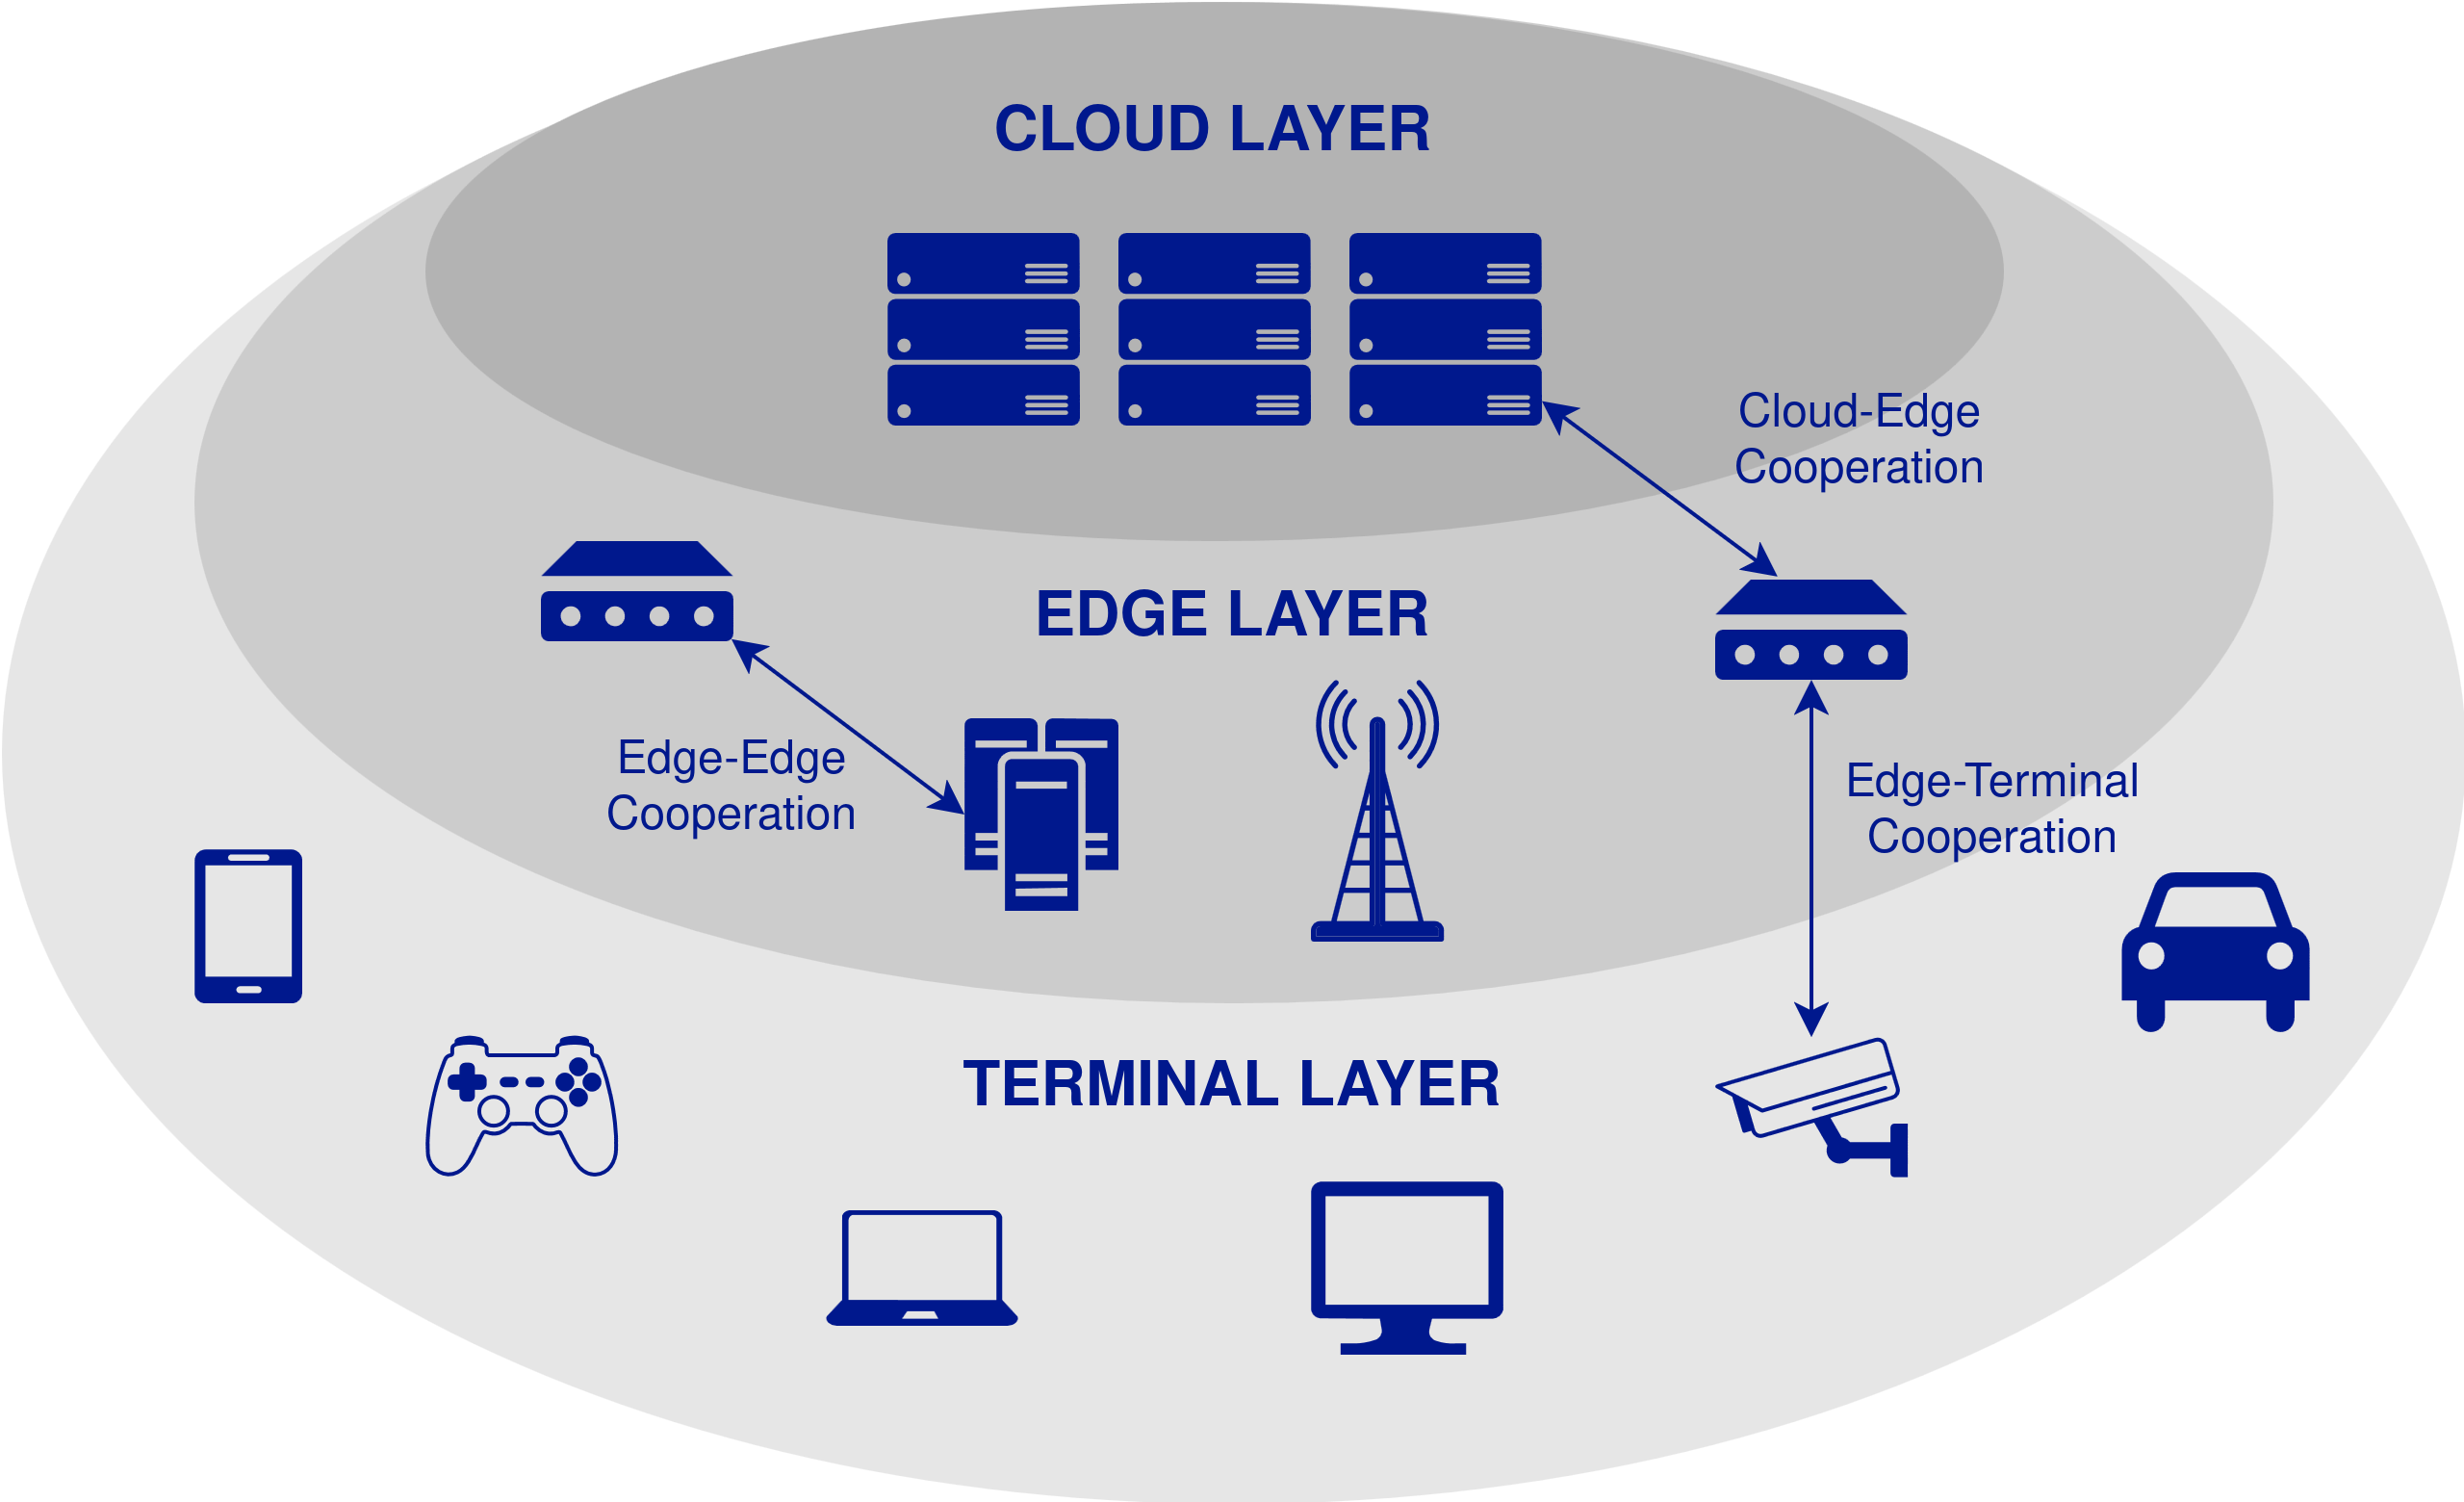
\includegraphics[width=0.8\linewidth]{figures/chapter1/3_layer_model.png}
    \caption{Three-layer model for representing Edge computing.}
    \label{fig:3_layer_model}
\end{figure}

Smarter service orchestration techniques are required to efficiently manage and allocate resources across geographically distributed Edge nodes, where heterogeneity, limited capacity, and dynamic workloads pose significant challenges. In such environments, energy efficiency becomes a critical concern, as Edge devices often operate under strict power constraints and may be deployed in locations with limited access to stable energy supplies. Consequently, service orchestration mechanisms must explicitly account for energy consumption, aiming to minimize power usage while preserving application performance and QoS\nomenclature{QoS}{Quality-of-Service}.

In parallel, the integration of renewable energy sources into Edge computing infrastructures has gained increasing attention as a means to improve the sustainability of Edge service provisioning. Edge nodes may be partially or fully powered by renewable sources such as solar or wind energy, often complemented by local energy storage systems (e.g., batteries) to mitigate the intermittency of energy generation. This introduces a new dimension to the orchestration problem, as decisions must consider not only computational and networking resources, but also the availability of harvested energy, battery state of charge, and energy forecasting. Energy-aware and renewable-aware orchestration strategies can use this data to shift workloads in space or time, prioritize nodes with a surplus of green energy, and reduce reliance on grid power.

\subsection{Network Function Virtualization}

NFV\nomenclature{NFV}{Network Function Virtualization} \cite{mulliganNetworkFunctionsVirtualisation2026} was introduced to change the way network services are designed, deployed, and managed by separating network functions from proprietary hardware. The concept was first formalized by the ETSI\nomenclature{ETSI}{European Telecommunications Standards Institute}, which initiated the NFV Industry Specification Group in 2012. ETSI NFV provides a standardized architectural framework, terminology, and reference models that have since become a foundation for both academic research and industrial implementations of NFV.

\subsubsection{Network Function Virtualization}

NFV is defined as the virtualization of network functions, such as firewalls, load balancers, intrusion detection systems, or packet gateways, that traditionally ran on dedicated hardware. In NFV, these functions are implemented as software instances, referred to as VNFs\nomenclature{VNF}{Virtual Network Function}, which run on non-dedicated computing platforms. By using Cloud-native principles, NFV enables greater flexibility, faster service deployment, reduced capital and operational expenditures, and improved scalability compared to hardware-based network infrastructures. More recently, VNFs are increasingly complemented or replaced by CNFs\nomenclature{CNF}{Cloud-Native Network Functions}, which are deployed as containers and managed using orchestration platforms such as Kubernetes.

\subsubsection{NFV Management and Orchestration}

To handle the complexity introduced by virtualized and distributed network functions, ETSI defined the NFV MANO\nomenclature{MANO}{Management and Orchestration} framework. NFV MANO is responsible for the lifecycle management of VNFs and network services, including instantiation, scaling, migration, healing, and termination. The MANO architecture is composed of three main components. First, the Virtualized Infrastructure Manager (VIM\nomenclature{VIM}{Virtual Infrastructure Manager}), which manages compute, storage, and networking resources. Then, the VNF Manager (VNFM), which controls the lifecycle of individual VNFs. Finally, the NFV Orchestrator (NFVO), which coordinates end-to-end network services across multiple VNFs and infrastructure domains. Together, these components enable automated and dynamic service orchestration in virtualized network environments. The global ETSI-NFV architecture is depicted in Fig. \ref{fig:nfv_architecture}.

\begin{figure}[!h]
    \centering
    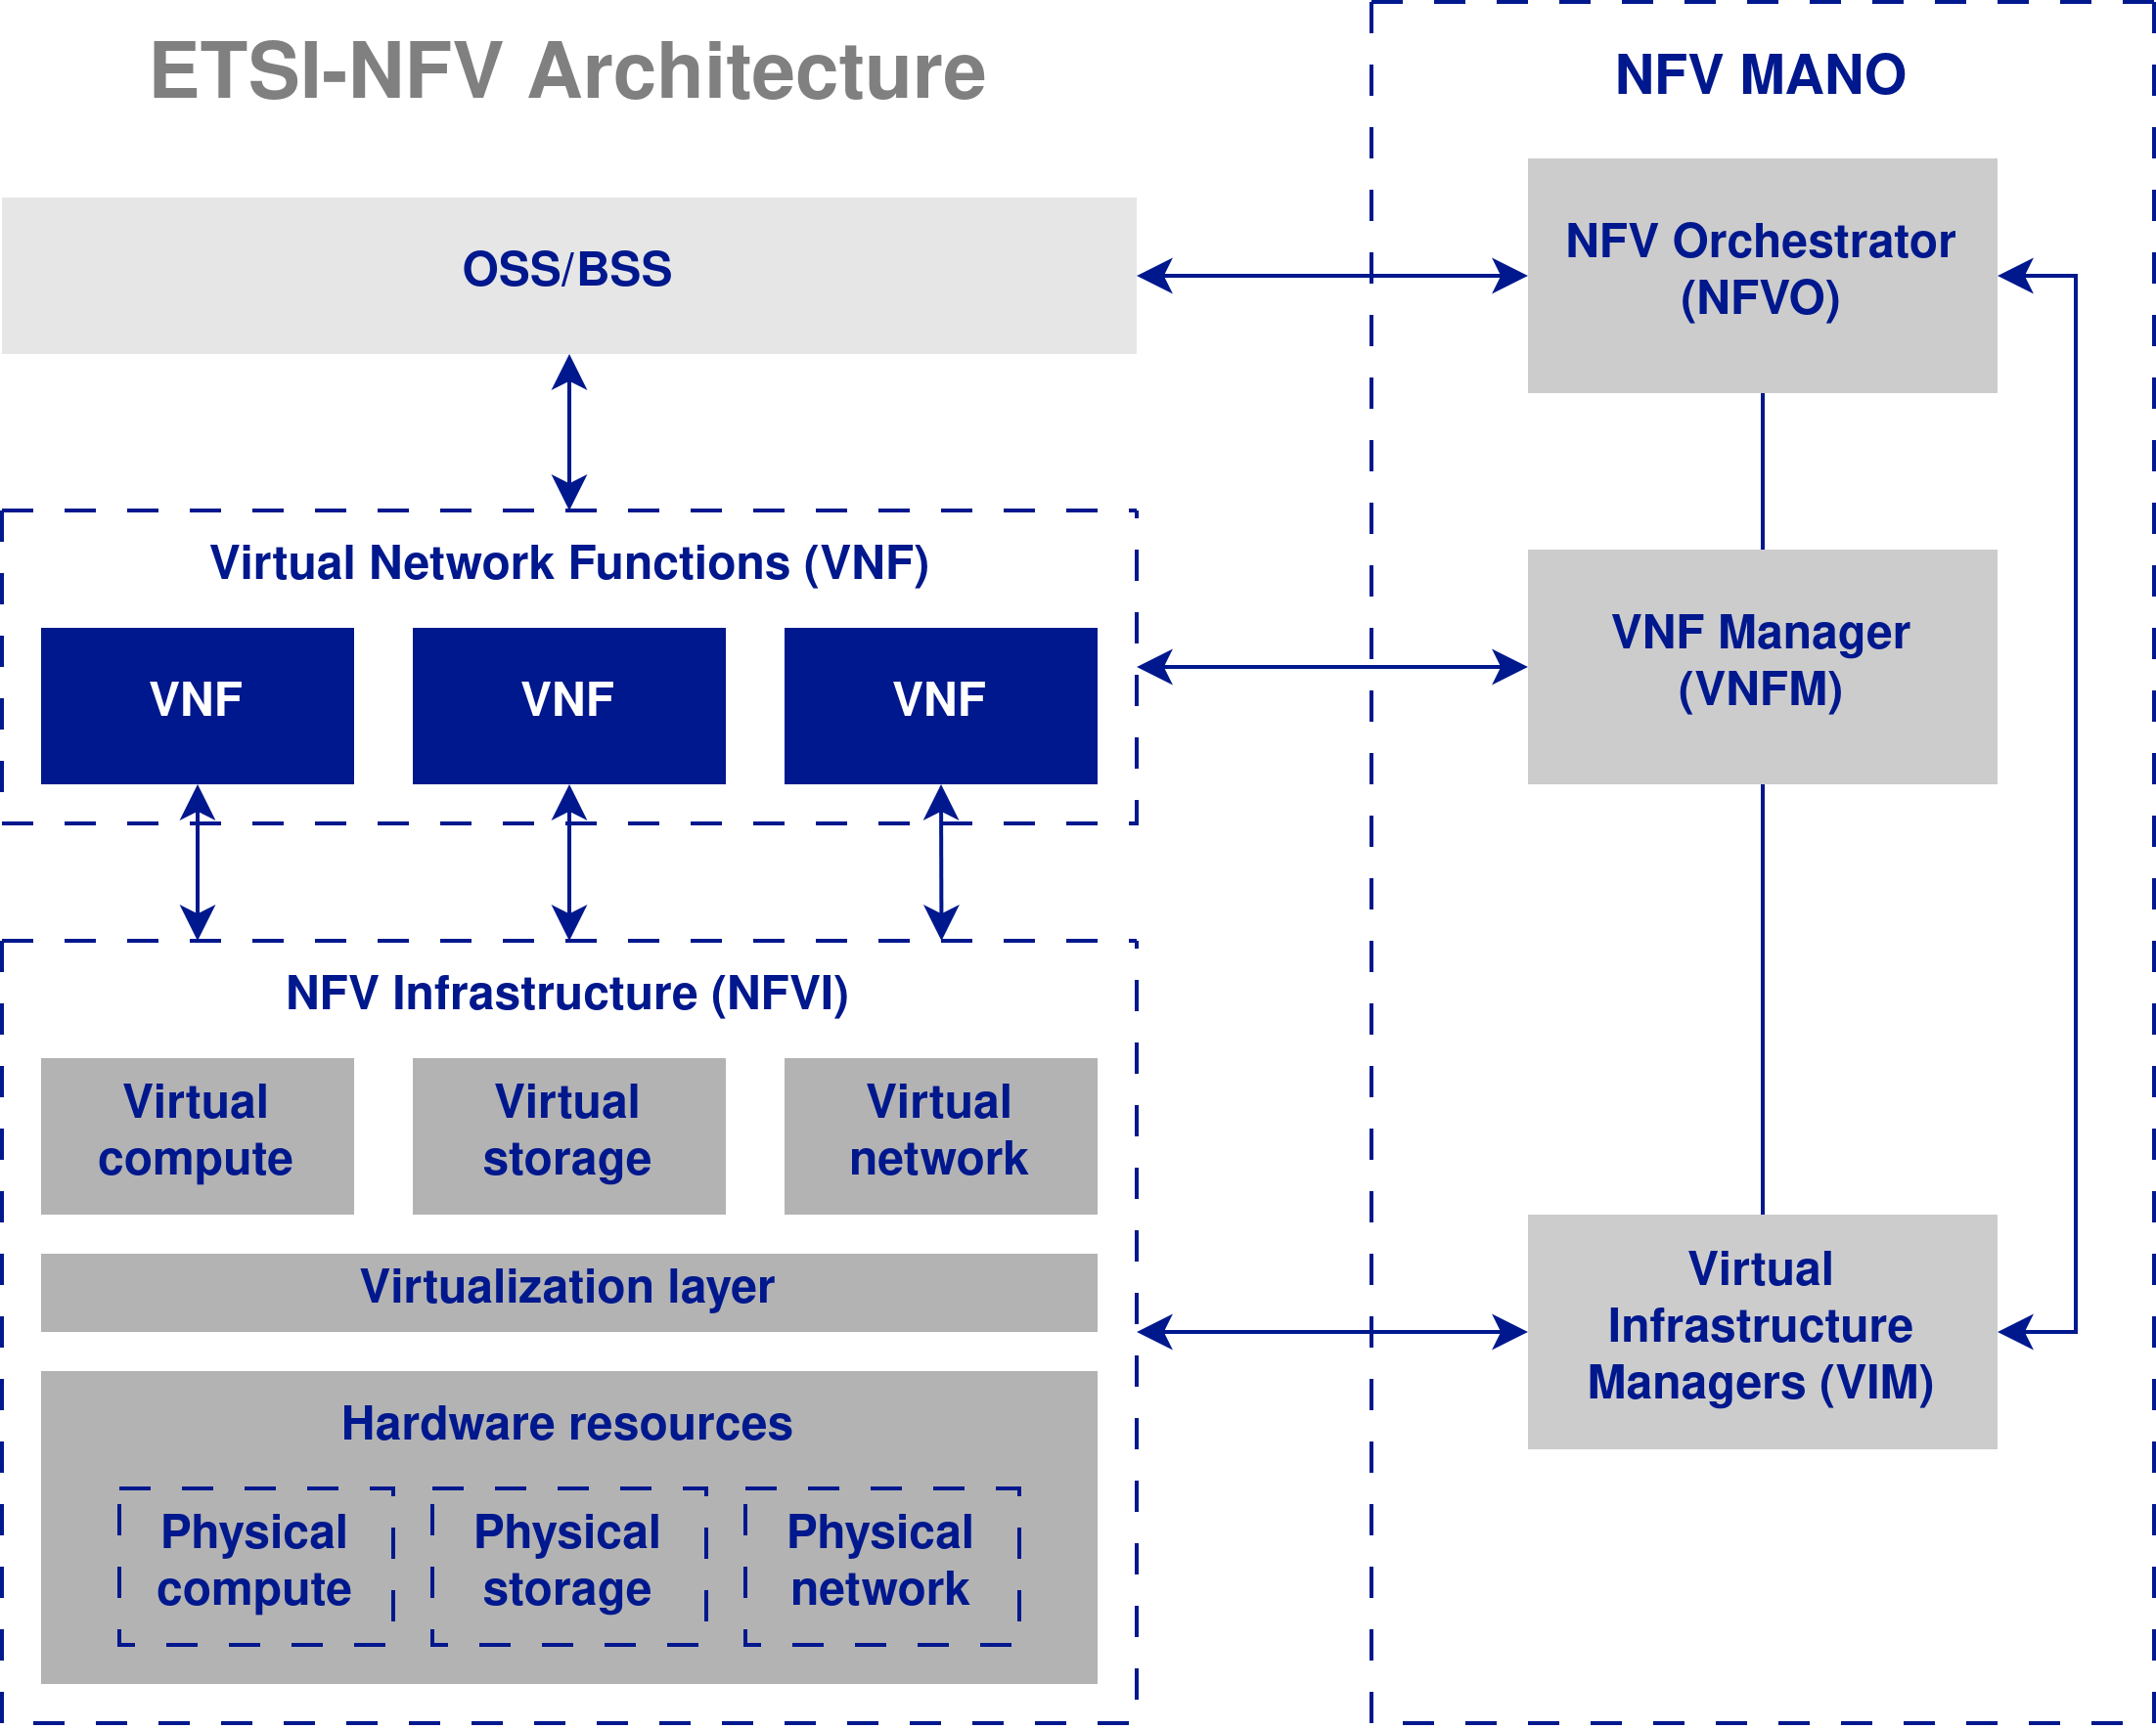
\includegraphics[width=0.8\linewidth]{figures/chapter1/nfv-architecture.png}
    \caption{ETSI NFV Architecture.}
    \label{fig:nfv_architecture}
\end{figure}

\subsubsection{Open Source MANO}

OSM\nomenclature{OSM}{Open Source MANO} \cite{Osm2026} is an open-source implementation of the NFV MANO framework, developed by ETSI, designed to be vendor-neutral and compliant with ETSI specifications. OSM provides a modular and extensible platform that supports the orchestration of both VNFs and CNFs across heterogeneous infrastructures, including VMs, containers, and hybrid environments. It integrates with multiple VIMs, such as OpenStack \cite{Openstack2026} and Kubernetes \cite{Kubernetes2026}, and offers support for multi-site and multi-domain deployments.

\section{Surveys on sustainable service orchestration strategies}

In recent years, Edge computing has emerged as a crucial paradigm for processing data closer to its source, significantly reducing latency and bandwidth usage. This paradigm shift necessitates advanced service orchestration techniques to efficiently manage and allocate resources across distributed Edge nodes. A key consideration in this context is the energy efficiency of these operations, as Edge devices often operate in resource-constrained environments where power consumption is a critical concern. Consequently, there is a growing focus on strategies to minimize energy consumption without compromising performance. In parallel, integrating renewable energy sources into Edge computing infrastructure has gained attention as a sustainable approach to reduce the carbon footprint of Edge services. This section is divided in three subsections to critically analyze existing studies and establish the research gap that motivates our work.

\subsection{Service orchestration for energy efficiency}

Existing literature on energy-efficient service orchestration can be categorized based on their scope and technical approach. However, a critical analysis reveals significant limitations in current approaches.

Several surveys focus exclusively on software-level optimizations while neglecting hardware-level energy management techniques. For instance, the authors in \cite{gaglianeseGreenOrchestrationCloudEdge2023} classify energy-aware approaches in the Cloud-Edge continuum but do not incorporate hardware management strategies such as DVFS or sleep mode operations. Similarly, the work presented in \cite{gitalEnergyManagementEdge2023} evaluates energy consumption metrics without addressing hardware-level optimizations and the survey in \cite{yangSurveyEnergyOptimization2023} focus only on task offloading and resource allocation strategies. Hardware management can contribute significantly to energy savings in Edge environments.

A portion of the literature addresses energy efficiency within specific application domains, limiting the generalization of findings. The authors of \cite{maoGreenEdgeAI2023} restrict their analysis to Edge AI applications, while in \cite{jiangEnergyefficientMechanismsSustainable2024} the focus is exclusively on Vehicular Fog Networks (VFN). The work in \cite{liuSurveyEdgeComputing2019} primarily studies existing Edge computing systems and open-source tools comparison. These domain-specific approaches, while valuable within their contexts, do not provide results applicable across diverse energy-efficient Edge computing scenarios.

Most critically, the majority of service orchestration studies operate under the assumption of traditional grid-powered infrastructure. The works in \cite{jiangEnergyAwareEdge2020} and \cite{congSurveyHierarchicalEnergy2020} address energy management and computation offloading without considering renewable energy integration. This represents a fundamental limitation because renewable energy alters orchestration strategies due to intermittency, varying power availability, energy storage constraints, and the need to manage multiple heterogeneous energy sources that traditional energy minimization approaches cannot adequately address.

\subsection{Renewable energy in Edge computing}

While renewable energy has gained attention in Edge computing research, current literature shows significant gaps in addressing its integration with service orchestration.

Several studies examine renewable energy in Edge computing contexts but fail to connect it with service orchestration strategies. The authors in \cite{israrRenewableEnergyPowered2021} explore renewable energy integration in 5G networks focusing on radio resource management, while the survey in \cite{rostirollaSurveyChallengesSolutions2022} provides extensive coverage of renewable energy in data centers but without Edge computing considerations. In \cite{pereraFogComputingSustainable2017}, the authors discuss Fog computing in smart cities but treat renewable energy and service orchestration as separate concerns. The work presented in \cite{sahRenewableEnergyHarvesting2020} addresses energy harvesting in wireless sensors without orchestration implications. These approaches do not study the synergies between renewable energy management and service orchestration.

When renewable energy is considered, it is typically constrained to specific use cases. The authors of \cite{guptaSurveyGreenUnmanned2022} limit their renewable energy discussion to solar power for roadside units and UAV applications, which may not translate to traditional Edge infrastructure scenarios.

A critical limitation in current literature is the predominant focus on energy harvesting for small-scale IoT devices rather than infrastructure-level renewable energy integration. The authors in \cite{shalaviEnergyEfficientDeployment2022} discuss energy-harvesting mobile Edge computing (EH-MEC) systems, but most cited works do not implement comprehensive renewable energy management. In \cite{benhamaidRecentAdvancesEnergy2022}, the authors concentrate on energy harvesting primarily for IoT devices, dividing discussions into energy harvesting and energy saving categories. This perspective overlooks crucial aspects of renewable energy integration including energy storage management, power prediction, grid interaction, and multi-source energy coordination that are essential for infrastructure-level implementations.

\subsection{Research gaps} \label{sec:research_gaps}

The critical analysis of existing literature reveals a fundamental research gap at the intersection of service orchestration and renewable energy integration in Edge computing. Current approaches have from three primary limitations:

\begin{itemize}
    \item Existing surveys typically address energy efficiency only in terms of reducing consumption during the orchestration process. The role and potential of renewable energy are often overlooked.
    \item In the few cases where renewable energy is considered, it is mainly viewed as a passive counterbalance to consumption. More advanced strategies, such as energy forecasting or the use of heterogeneous energy sources, are rarely explored in the service orchestration scenarios.
    \item Most renewable energy literature reviews in Edge computing focus on energy harvesting for IoT devices, while the orchestration strategies that integrate renewable energy at the infrastructure or data center level are largely neglected.
\end{itemize}

\section{Sustainability in service reconfiguration}

In dynamic environments characterized by variable renewable energy generation and potential node departures, service reconfiguration is essential to maintain system performance and sustainability. Two main categories of reconfiguration strategies can be identified in the context of sustainable orchestration. First, \emph{behavioral} reconfiguration strategies focus on adapting services by scaling, activating, or deactivating internal functions of deployed services based on current energy availability and workload demands. Second, \emph{structural} reconfiguration strategies involve modifying the placement of services across the infrastructure, migrating components to nodes with better energy profiles or lower risk of departure. While both strategies are essential, structural reconfiguration is particularly relevant in scenarios where node departures are unpredictable, as it allows for proactive adjustments to service placements to enhance robustness.

\subsection{Service Placement \& Placement reconfiguration}

Several works have addressed service placement in Cloud and Edge environments. In \cite{chenEnergyefficientServiceDeployment2024a}, the authors consider service deployment across Edge servers by accounting for geographical coordinates, user distribution patterns, and service preferences. In \cite{liangSustainableVirtualNetwork2024b}, the placement of VNFs in mobile Edge networks is studied, where VNFs are structured in service function chains (SFCs)\nomenclature{SFC}{Service Function Chain} for each user, and traffic must flow through the VNFs in sequence. In \cite{ahvarDECADynamicEnergy2021}, application components are distributed across different Edge clouds, and because components communicate with each other, placement decisions directly affect energy consumption. The authors of \cite{spinelliMigrationPathGreen2022} focus on job placement and migration in a MEC system, where each job is associated with revenue and cost. They show that migration decisions, while costly in terms of time and energy, can improve overall energy efficiency and QoS in contexts such as game session management. In \cite{fangResourceAllocationStrategy2020b}, VM migration is analyzed in the context of user mobility, with the goal of minimizing energy consumption as users move across the network. Similarly, container migration is studied in \cite{perinEASEEnergyAwareJob2023b}, where energy costs are considered, and migration decisions are only performed if they provide a net gain in energy efficiency. In \cite{guServiceManagementEnergy2023b}, the focus is on service management to reduce migration costs, while \cite{shenBackupBatteryAllocation2023} examines workload migration for balancing workload distribution, operational costs, and QoS trade-offs.

\subsection{Sustainability \& Robustness}

Only a small number of works explicitly consider renewable energy in this context. In \cite{liangSustainableVirtualNetwork2024b}, renewable energy (solar) is introduced in vehicular networks, while \cite{guServiceManagementEnergy2023b} explores solar and wind energy in Edge computing. Both models integrate batteries to store intermittent renewable energy. While several papers do account for renewable energy, such as \cite{guServiceManagementEnergy2023b,spinelliMigrationPathGreen2022,ahvarDECADynamicEnergy2021}, only \cite{haqueProvidingGreenSLAs2013} address it from a service-centered perspective. In that work, the concept of a green service level agreement (SLA)\nomenclature{SLA}{Service Level Agreement} is introduced, where services must consume at least a given percentage of energy from renewable sources. In addition to renewable energy, robustness to node departure is another important concern. Indeed, infrastructures in Edge computing are subject to various types of node departures, which can be voluntary, e.g. mobility, user-driven shutdowns, resource withdrawal, or non-voluntary, e.g. crash failures, connectivity loss, energy shortages, environmental hazards. To ensure service continuity, it is crucial to implement measures that mitigate the impact of these departures, especially when they cannot be predicted in advance. In \cite{yuMicroserviceResilienceDeployment2022}, a node diversity metric is proposed to evaluate microservice resilience to failures. The authors of \cite{chengResilientEdgeService2024} propose an uncertainty model for node failures in Edge computing. However, these approaches do not consider renewable energy, even though the intermittence of renewable sources and node departure risks are closely related.

\subsection{Prediction mechanisms}

Since renewable energy is intermittent, prediction mechanisms are necessary. Few works have addressed this problem. In \cite{perinEASEEnergyAwareJob2023b}, energy harvested from photovoltaic systems is estimated within a time window, with future power values modeled as Gaussian random variables. A receding horizon approach is then applied to solve scheduling decisions, allowing optimization of task execution based on expected energy availability. In \cite{haoEnergyAllocationTask2023c}, solar energy prediction is based on meteorological data, considering variables such as sunlight intensity, surface area, and conversion efficiency, with solar radiation as the main source of uncertainty. Similarly, \cite{angelajennifasujanaFogIntelligenceEnergy2024a} rely on meteorological data to forecast both light and power demand for solar-powered street lamps using quantile regression. In our contribution, we chose not to use meteorological data, as it might not always be available, and instead rely solely on historical power output and workload traces. We use a Sequence-to-Sequence (Seq2Seq) model \cite{sutskeverSequenceSequenceLearning2014} to predict both renewable energy generation and workload demands. Seq2Seq models have already been applied to energy-related forecasting tasks, such as energy consumption in industrial processes \cite{howindModelingEnergyConsumption2023} and day-ahead power generation scheduling in island power systems \cite{nishtarSeq2SeqBasedDayAheadSchedulingSCUC2024}.
  
\section{Practical implementation with NFV MANO} 

\subsection{NFV MANO Solutions}

\subsection{Cloud Platforms for NFV MANO}

\subsection{Energy-Aware NFV}

\section{Conclusion}

Our work is around three axes.

First, from gaps identified in Section \ref{sec:research_gaps}, we provide a new analysis of service orchestration strategies specifically designed for renewable energy-powered Edge computing environments. Unlike existing work that treats energy minimization and renewable energy as separate concerns, we examine orchestration strategies that explicitly account for renewable energy characteristics including intermittency, storage constraints and multi-source energy management. Our focus on orchestration strategies rather than optimization algorithms distinguishes this work from existing surveys that primarily consider algorithmic solutions. We analyze how renewable energy integration necessitates new orchestration strategies that go beyond traditional energy minimization by studying energy storage management, power prediction, renewable energy source coordination and grid interaction aspects that remain largely unexplored in current literature. This approach not only fills existing research voids but also provides a foundation for developing more sustainable and efficient Edge computing environments that can effectively use renewable energy sources through intelligent service orchestration.

Our second contribution addresses the problem of service placement and service placement reconfiguration. Unlike most existing works, which rely on battery-dependent systems, we focus on a battery-free infrastructure, an on-spot energy strategy, since batteries introduce high operational costs and require frequent replacement. In out scenario, all nodes are connected to the power grid, eliminating the need for batteries. Additionally, we integrate both sustainability and robustness as key optimization objectives, an approach that remains unexplored despite their complementary nature in renewable energy-enabled Edge systems. To further enhance our placement and placement reconfiguration algorithms, we employ a Seq2Seq model to forecast renewable energy generation and workload demand, enabling us to optimize our selected metrics more effectively.

\ifdefined\included
\else
\bibliographystyle{acm}
\bibliography{These}
\end{document}
\fi

\ifdefined\included
\else
\documentclass[a4paper,11pt,twoside]{StyleThese}
\include{formatAndDefs}
% fallback si compilation standalone
\providecommand{\acs}[1]{#1}
\providecommand{\minitoc}{}
\providecommand{\dominitoc}{}
\providecommand{\faketableofcontents}{}
\hbadness=10000
\sloppy
\begin{document}
\setcounter{chapter}{1} %% Numéro du chapitre précédent ;)
\dominitoc
\faketableofcontents
\fi

\chapter{Etat de l'art des attaques 5G}
\minitoc

% (PB1 : Manque d’information de la part des opérateurs sur ce qui est réaliste ou non)
Les opérateurs de télécommunications communiquent très peu sur la nature de leurs implémentations ainsi que sur les attaques auxquelles ils sont confrontés. Cette « sécurité par l’obscurité » limite l’émergence de menaces opportunistes et préserve des avantages concurrentiels. Toutefois, elle constitue également un frein important pour la recherche académique. En l’absence de données empiriques et de retours d’expérience concrets, de nombreux travaux proposent des scénarios d’attaque théoriques sans disposer de cadre de référence solide, rendant difficile l’évaluation de leur réalisme et de leur applicabilité dans des environnements opérationnels.

% (PB2 : La définition d’une attaque 5G est flou à cause de mauvaise caractérisation)
Ce flou de l'état de l'art en matière de réalisme est accentué par une caractérisation parfois insuffisante des attaques dans la littérature scientifique. Certains travaux reposent sur des modèles d’attaquants incomplets, des hypothèses peu explicites ou encore des expérimentations menées sur des implémentations open source trop peu matures. Bien qu’il existe des cadres méthodologiques dédiés à la caractérisation des attaques tels que FIGHT, ceux-ci présentent encore des limites et demeurent, à notre connaissance, très peu adoptés dans l’état de l’art. Cette situation contribue à entretenir une certaine ambiguïté quant à la définition et à la classification des attaques réellement pertinentes dans le contexte de la 5G.

% (PB3 : Proposition d’une nouvelle méthode de classification innovante)
Par ailleurs, les approches traditionnelles de détection d’anomalies reposent majoritairement sur l’analyse de flux à grande échelle, fondée sur des indicateurs volumétriques. Cependant, la softwarisation des réseaux 5G rapproche ces infrastructures de systèmes distribués complexes, ce qui nécessite désormais une analyse plus fine, notamment au niveau des paquets. Afin de répondre à ce changement de paradigme, nous proposons une nouvelle catégorisation en trois classes d'attaques : sémantiques, séquentielles et topologiques, chacune présentant des problématiques spécifiques en matière de détection.

\section{Les plateformes open source comme une approximation du réel}

\section{Exemples de mécanismes de sécurité négligés par l’état de l’art}

\section{Distinction entre les attaques réalistes et les hypothèses irréalistes }
\subsection{Attaques spécifiques aux implémentations}
\subsection{Attaques visant des failles dans les standards}

\section{Les limites de MITRE en tant que framework de catégorisation}
\subsection{Absence de techniques bien connues}
\subsection{Status incorrects des techniques}
\subsection{Manque de détails sur les caractéristiques des techniques}
\subsection{Pourquoi et comment caractériser nos attaqus}

\section{Nouvelle classification propre aux enjeux de détections}
\subsection{Anomalies sémantiques}
\subsection{Anomalies séquentielles}
\subsection{Anomalies topologiques}

\section{Conclusion}

\ifdefined\included
\else
\bibliographystyle{acm}
\bibliography{These}
\end{document}
\fi

\ifdefined\included
\else
\documentclass[a4paper,11pt,twoside]{StyleThese}
\include{formatAndDefs}
% fallback si compilation standalone
\providecommand{\acs}[1]{#1}
\providecommand{\minitoc}{}
\providecommand{\dominitoc}{}
\providecommand{\faketableofcontents}{}
\usepackage{subcaption}
\hbadness=10000
\sloppy

\begin{document}
\setcounter{chapter}{2} %% Numéro du chapitre précédent ;)
\dominitoc
\faketableofcontents
\fi

\chapter{Détection d’anomalie multi-domaines}
\minitoc

%PB1 : Les méthodes proposées actuellement pour la détection d’anomalie sont pas adaptés
Le passage aux réseaux 5G s’accompagne d’un changement de paradigme majeur, caractérisé par une architecture distribuée et une complexification des interactions entre entités. Par ailleurs, l’émergence d’anomalies sémantique, séquentielle et topologique impose de nouvelles exigences en matière d’analyse. Dans ce contexte, il devient nécessaire non seulement d’adopter une analyse fine au niveau des paquets, mais également de prendre en compte le contexte dans lequel s’inscrivent les échanges. Or, cette problématique reste relativement récente dans le domaine des télécommunications, et les méthodes actuelles de détection d’anomalies apparaissent inadaptées à ce nouveau paradigme.

%PB2 : Pourquoi la formalisation de notre problème en GNN Dynamique nous parait pertinent
Dans ce contexte, nous proposons de représenter les échanges au sein des réseaux 5G sous la forme d’un graphe dynamique, permettant de capturer à la fois les interactions entre les différentes entités du réseau ainsi que l’évolution de ces interactions dans le temps. ette formalisation nous permet d’exploiter des techniques issues du domaine des GNN intrinsèquement adaptées à l’analyse des interactions complexes. Nous nous intéressons plus particulièrement aux GNN dynamiques, qui intègrent nativement la dimension temporelle.

%PB3 : Pourquoi le NLP est une bonne piste si on veut traiter une quantité indénombrable de données mais on ne l’a pas creusé

\section{Objectifs et cadre de détection}
% Scope = trafic de contrôle
Dans ces travaux, nous nous plaçons du point de vue de l’opérateur d’un réseau 5G et nous nous intéressons à la détection d’anomalies en nous concentrant exclusivement sur le trafic de contrôle échangé entre les entités du réseau, qu’il s’agisse du cœur de réseau ou du RAN. Le trafic utilisateur n’est pas pris en compte, car il ne présente pas de spécificités propres à l’architecture 5G et ne relève pas de la responsabilité directe du fournisseur d'accès réseau.

% Accès à tout le trafic
En se plaçant du point de vue de l’opérateur, nous supposons que celui-ci possède l’ensemble des NF et dispose d’un accès complet au trafic de contrôle. Dans l’architecture 5G, la fonction Service Communication Proxy (SCP) agit comme un intermédiaire dans les échanges entre les différentes NF, notamment pour le routage des requêtes et la vérification des autorisations d’accès. Dans ce contexte, il est raisonnable de considérer que l’opérateur peut observer l’intégralité du trafic de contrôle en déployant des sondes au niveau des SCP, qui constituent des points d’observation privilégiés des interactions entre NF. 

% Chiffrement
Ce trafic est généralement chiffré, par exemple via TLS sur le SBI ou via IPsec pour certains canaux, tels que N3 ou N4, reposant sur des protocoles spécifiques à la 5G. Cependant, en adoptant le point de vue de l’opérateur, nous supposons disposer des clés de chiffrement nécessaires pour accéder au contenu de ces échanges en clair.

% Performances
L’objectif serait de pouvoir exécuter nos modèles de détection en temps réel. Malgré les débits élevés offerts par la 5G, le volume de données est majoritairement porté par le trafic utilisateur, qui n’entre pas dans le périmètre de cette étude. À l’inverse, le trafic de contrôle est principalement composé de messages liés aux changements d’état des entités du réseau, qu’il s’agisse d’UE ou de NF, et ont une fréquence d’occurrence plus modérée. Par conséquent, bien que le surcoût induit par nos modèles puisse avoir un impact sur les performances, il est raisonnable de supposer que les ressources disponibles sont suffisantes pour permettre un traitement en temps réel, notamment grâce à l’exploitation de techniques d’optimisation et de parallélisation.

% Remédiation
La remédiation des anomalies détectées ne relève pas du périmètre de ce travail et est considérée comme une brique fonctionnelle distincte. Nous nous concentrons exclusivement sur la détection et les alertes générées par notre système ont vocation à être exploitées de manière similaire à celles produites par un système de détection d’intrusion (IDS) classique. Elles peuvent ainsi conduire, par exemple, à des ajustements des règles de firewall ou à des modifications de l’architecture réseau.

% Vrais objectifs
L’objectif de ces travaux n’est pas de concevoir un système de détection absolu et entièrement autonome. En effet, une anomalie ne constitue pas nécessairement le signe d’une activité malveillante et peut résulter d’une mise à jour, d’une erreur de configuration ou encore d’une interconnexion avec un système tiers, comme dans le cas du roaming. Dans ce contexte, la distinction entre une anomalie bénigne et une attaque de type zero-day requiert in fine une expertise humaine. Par conséquent, l’un des aspects essentiels de nos travaux est de proposer un système interprétable, venant complémenter une expertise humaine plutôt que de la remplacer.

\section{Etat de l’art de la détection d’anomalies}
\subsection{Approche historique dans les réseaux traditionnels}
La détection d’attaques au sein des réseaux est historiquement assurée par des systèmes de détection d’intrusion (IDS). Ces systèmes reposent généralement sur une analyse du trafic agrégé sous forme de flux, plutôt qu’au niveau des paquets individuels. Cette approche permet d’extraire des métriques globales et d’effectuer des analyses de volumétrie, par exemple afin de détecter des variations significatives du volume de trafic ou repérer des signatures d'attaques connues.

% Rule Based
Parmi les IDS les plus connus on retrouve Snort \cite{snort}, Zeek \cite{zeek} et Suricata \cite{suricata}, qui reposent sur des règles prédéfinies pour identifier des motifs (aussi appelés signatures) d’attaques spécifiques dans le flux réseau. Ce sont la plupart du temps des outils open source qui bénéficient d'une large communauté qui contribue à l'enrichissement de leur base de signatures. 

% ML Supervisé
Par ailleurs, des approches fondées sur l’apprentissage automatique supervisé ont également été proposées pour la détection d’intrusion, notamment à l’aide de réseaux bayésiens \cite{bayesian}, de machines à vecteurs de support (SVM) \cite{svm} ou encore d’arbres de décision \cite{decision_tree}. Ces méthodes présentent l’avantage d’être relativement transparentes, interprétables et efficaces pour détecter des attaques déjà connues.

% Limites + Conclusion
Néanmoins, les modèles de détection supervisé et rule based restent ultimement limités à la détection d’attaques déjà connues et ne permettent pas de considérer des comportements anormaux au niveau paquet ou des attaques zero-day. Or, il existe une grande variété de formes de cyberattaques et de nouvelles menaces émergent régulièrement. Cette diversité est amplifiée dans un système complexe tel que la 5G et il devient inenvisageable de dresser une liste exhaustive des menaces courantes et à venir. De fait, les approches non supervisées paraissent plus adaptées car elles permettent d’identifier des comportements anormaux, même inconnus, en se fondant sur des déviations par rapport aux comportements normaux présentés lors de l'entrainement. 
% Non Supervisé

% K-Means
Parmi les approches non supervisées, Münz et al. \cite{kmeans} proposent, par exemple, de découvrir des motifs anormaux en adaptant l’algorithme K-Means au trafic réseau, permettant ainsi de regrouper les données en fonction de leur similarité sans nécessiter d’étiquettes. Néanmoins, les caractéristiques utilisées en entrée restent relativement limitées et se restreignent notamment au nombre de paquets, au volume d’octets ainsi qu’aux adresses source et destination. Une telle approche permet d’identifier des motifs liés à la volumétrie et, par conséquent, de détecter certains types d’attaques par déni de service (DoS). Toutefois, comme elle ne prend en compte ni le contenu sémantique des paquets ni le contexte des échanges, elle demeure insuffisante pour détecter des attaques plus subtiles.

% Markov
Ariu et al. \cite{markov} proposent quant à eux d'utiliser des modèles de Markov cachés afin de modéliser le trafic réseau sous forme de séquences d’octets. Ces modèles apprennent des probabilités de transition à partir de trafic bénin, puis évaluent dans quelle mesure un trafic observé s’en écarte. Cependant, les séquences considérées sont limitées à des fenêtres de taille relativement réduite, ce qui empêche la capture de dépendances temporelles à long terme. De plus, cette approche ne permet pas de modéliser explicitement les interactions entre paquets.

\subsection{Apprentissage profond appliqué aux réseaux 5G}

% Spécifique 5G
Parmi les travaux de détection spécifiques à la 5G, Kale et al. \cite{ensemble} proposent d’utiliser des réseaux de neurones convolutionnels (CNN) en considérant les octets d’un paquet comme une image sur laquelle sont ensuite étudiées des variations structurelles. Les modèles CNN obtiennent de très bonnes performances dans de nombreux domaines, y compris dans des tâches qui ne relèvent pas intrinsèquement de la vision par ordinateur. Toutefois, comme ils n’interprètent pas le contenu sémantique des données, leur capacité de détection se limite à un sous-ensemble d’attaques sémantiques dans lesquelles les valeurs s’écartent fortement du trafic normal. Ils ne permettent donc pas de détecter des variations légères de valeurs d'identifiants comme les adresses IP ou les IMSI. De plus, le travail présenté par Kale et al. se concentre uniquement sur la détection sémantique et ne prend pas en compte le contexte des échanges. Lam et al. \cite{cnn} ajoutent un contexte temporel à leur CNN en alimentant ses sorties dans un réseau de neurones récurrent RNN. Cependant, en plus de ne pas être satisfaisant sur le domaine sémantique, leur modèle ne prend pas en compte l’identité des acteurs impliqués dans les échanges et n’est donc pas capable de détecter des attaques relationnelles.

AutoGuard \cite{autoguard} et ADSeq-5GCN \cite{adseq} formalisent les échanges réseau sous forme de séquences d’interactions entre entités du réseau et utilisent également des RNN afin de capturer les dépendances temporelles. Leurs approches intègrent l’identité des entités communicantes, ce qui leur permet de prendre en compte, dans une certaine mesure, le contexte topologique des interactions à court terme. Cependant, elles rencontrent des difficultés à modéliser efficacement les dépendances relationnelles lorsque les interactions sont éloignées dans le temps. De plus, le principal problème est que leur formalisme n’intègre aucunement le contenu des paquets et ne considère donc aucunement la dimension sémantique. 5GCGuard \cite{5GCGuard} tente de pallier cette limitation en enrichissant leurs séquences par l’intégration de l’URL associée à chaque message. Bien qu'elle apporte une information sémantique supplémentaire, cette approche demeure très limitée car l’information propre à l'URL ne représente qu’une fraction du contenu réel des paquets et n'est applicables qu'au traffic HTTP.

\begin{figure}[h]
\centering
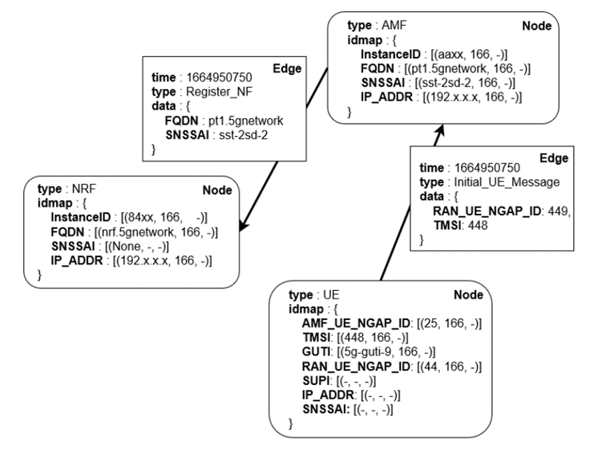
\includegraphics[width=0.7\linewidth]{figures/chapter3/prov5GC.png}
\caption{Trafic de contrôle 5G formalisé par Prov5GC \cite{prov5G} en tant que graphe de provenance}
\label{fig:prov5GCs}
\end{figure}

% Prov5G
Prov5GCC \cite{prov5G} propose de son côté de représenter le trafic sous forme de graphe de provenance. Dans cette représentation, illsutrée sur la figure \ref{fig:prov5GCs}, les nœuds correspondent aux entités du réseau et chaque message échangé entre ces entités est modélisé par une arête, à laquelle est associé le contenu du paquet. La formalisation en graph est particulièrement adaptée à l’analyse topologique des interactions du réseau. Cependant, elle ne modélise pas explicitement la dimension temporelle des échanges, ce qui restreint la capacité à capturer l’évolution dynamique des interactions. De plus, le fait d’agréger le payload au niveau des arêtes limite fortement l’exploitation de l’information contenue dans les paquets. Dans leur cas la payload est utilisé par un algorithme de détection heurisitique spécifique à chaque attaque, ce qui rend l’approche relativement lourde et peu adaptée à des environnements complexes.

\begin{figure}[h]
\centering
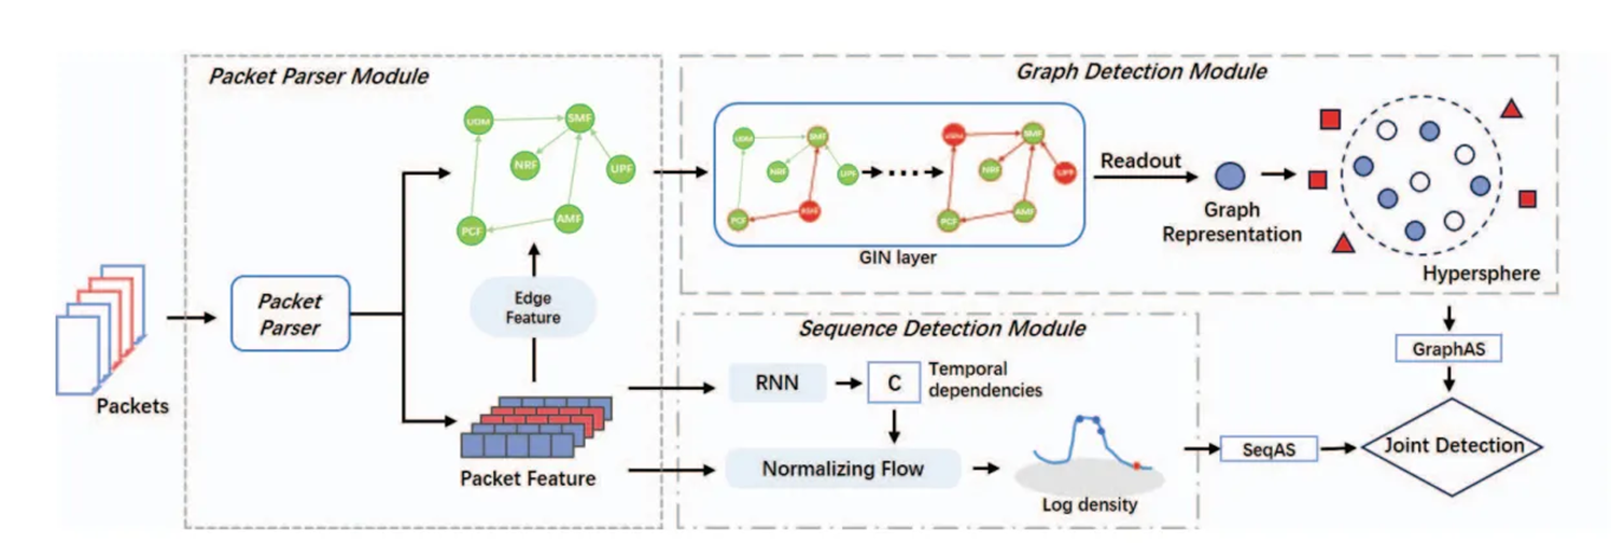
\includegraphics[width=\linewidth]{figures/chapter3/GSAD.png}
\caption{Pipeline de GSAD \cite{gsad} représentant leur formalisation ainsi que les trois modules de détections traitant respectivement les dimensions sémantique, séquentielle et topologique}
\label{fig:gsad}
\end{figure}


% GSAD
GSAD \cite{gsad} propose également de formaliser les données sous forme de graphe, de manière similaire à Prov5GC \cite{prov5G}. La principale différence réside dans la représentation du contenu des arêtes. Au lieu de l’encoder sous forme de dictionnaire monolithique, les auteurs le transforment en flux d’octets structuré comme une image. Cette représentation leur permet d’utiliser un CNN pour encoder chaque paquet et analyser sa dimension sémantique. Les représentations sémantiques sont ensuite injectées dans un GNN afin de modéliser les interactions entre les paquets, puis dans un RNN pour capturer les dépendances temporelles. À notre connaissance, GSAD \cite{gsad} est la seule approche de détection d’anomalies 5G basée sur l’apprentissage profond qui considère simultanément les trois dimensions de détection. La principale limite de leur approche réside dans le fait que, comme évoqué précédemment, les CNN ne permettent qu’une analyse relativement superficielle de la dimension sémantique des paquets. La Figure~\ref{fig:gsad} illustre l’architecture générale du pipeline proposé par GSAD et met en évidence les trois composantes du modèle correspondant respectivement aux trois dimensions.


\begin{table}[h]
\centering
\begin{tabular}{lccc}
\hline
\textbf{Référence} & \textbf{Sémantique} & \textbf{Séquentiel} & \textbf{Topologique} \\
\hline
Kale et al. \cite{ensemble}         & Oui      & Non      & Non \\
Lam et al. \cite{cnn}               & Oui      & Oui      & Non \\
AutoGuard \cite{autoguard}          & Non      & Oui      & Partiel \\
ADSeq-5GCN \cite{adseq}             & Non      & Oui      & Partiel \\
5GCGuard \cite{5GCGuard}            & Non      & Oui      & Partiel \\
Prov5GC \cite{prov5G}               & Partiel  & Non      & Partiel \\
GSAD \cite{gsad}                    & Partiel  & Partiel  & Oui \\
\hline
\end{tabular}
\caption{Comparaison des approches de l'état de l'art de détection d'anomalies 5G selon les dimensions considérées}
\label{tab:sota_comparison}
\end{table}

% Conclusion 
Le tableau \ref{tab:sota_comparison} résume les différentes approches de détection d’anomalies dans les réseaux 5G, en mettant en évidence les dimensions sémantique, temporelle et topologique prises en compte par chacune d’elles. L’état de l’art montre que peu d’approches considèrent simultanément les trois dimensions. Les approches basées sur les GNN apparaissent particulièrement adaptées pour modéliser les interactions entre entités. À l’inverse, aucune des modélisations proposées ne semble réellement adaptée au traitement du contenu sémantique des paquets, celui-ci étant le plus souvent considéré comme un bloc monolithique. Dans ce contexte, nous proposons de représenter le contenu des paquets de manière plus fine en décomposant leurs paramètres en nœuds indépendants. 

\subsection{Comparaison aux techniques utilitées dans les systèmes distribués}
La 5G partage de nombreuses caractéristiques architecturales avec les systèmes distribués modernes. Lorsque l’on s’intéresse à la littérature portant sur la détection d’anomalies dans ce domaine\cite{dist_gnn2}, on constate que les approches proposées reposent principalement soit sur le Federated Learning (FL), afin d’exploiter la nature distribuée des infrastructures, soit sur l’analyse de logs systèmes.

Les approches basées sur le FL, telles que DioT\cite{diot} ou VFL\cite{vfl}, mettent particulièrement en avant les avantages de la fédération pour les systèmes distribués, notamment en matière de passage à l’échelle, de confidentialité et de décentralisation de l’apprentissage. Cependant, leur contribution porte principalement sur le mécanisme de fédération lui-même. Les modèles utilisés restent relativement classiques et ne considèrent généralement qu’une partie des dimensions nécessaires à une détection complète des anomalies. DioT\cite{diot} s’appuie par exemple sur des GRU pour modéliser les dépendances temporelles, tandis que VFL\cite{vfl} exploite GraphSAGE afin de capturer les relations structurelles entre entités.

Les approches basées sur les logs telles que \cite{dist_log1,dist_log2} qui sont très utilisées dans les systèmes distribués présentent également plusieurs limitations. Bien qu’elles permettent d’observer l’activité du système à un haut niveau, les logs constituent une représentation indirecte et partielle des événements réseau. Ils dépendent fortement des implémentations logicielles et peuvent contenir du bruit, des informations manquantes ou des incohérences. Certains événements ou comportements anormaux peuvent ainsi ne jamais être journalisés, limitant la capacité de détection.

Enfin, un grand nombre de travaux restants s’appuient sur des GNN \cite{dist_gnn1,dist_gnn2}, ce qui confirme que la formalisation en graphe est particulièrement adaptée à la modélisation des interactions au sein des systèmes distribués.

\section{Méthodologie de formalisation}
Nous avons vu que le formalisme de graphe était particulièrement adapté à la modélisation de notre problème et qu’il permettait d’intégrer simultanément les dimensions sémantique, temporelle et topologique, comme l’a notamment montré GSAD. La principale différence avec leur formalisation est qu'au lieu de représenter le contenu des paquets comme un bloc monolithique associé à une arête, nous proposons de le décomposer en nœuds indépendants. Nous détaillons à présent notre méthodologie de formalisation. Nous commencerons par l’extraction des caractéristiques à partir du trafic de contrôle, puis nous présenterons leur transformation en graphes adaptés à une analyse par GNN.

\subsection{Extraction des features depuis la payload applicative}
Comme notre objectif est principalement d’analyser le contenu applicatif des paquets, nous extrayons la payload ainsi que l’ensemble des champs disponibles pour chaque paquet. Les seules informations non applicatives conservées concernent la couche IP, utilisées comme identifiant afin de discriminer les différentes entités du réseau. Cette approche n’est pas idéale, car elle est sensible au \textit{spoofing}. Toutefois, dans un cadre opérationnel, ces identifiants pourraient être remplacés par des mécanismes plus robustes, tels que des empreintes ou des hash représentant les entités de manière unique.

Pour récupérer le contenu des payloads, nous utilisons \textit{Scapy}, qui permet de parser les paquets réseau et de générer, pour chacun d’eux, une représentation sous forme de dictionnaire associant les champs à leurs valeurs respectives.

Un des problèmes rencontrés concerne certains paquets, notamment HTTP/2, qui contiennent principalement des structures JSON fortement imbriquées, ce qui introduit une complexité supplémentaire. La conservation explicite du chemin d’imbrication dans notre formalisme modifierait fortement la structure du graphe et accorderait une importance excessive à cette information. L’imbrication est utile pour différencier des paramètres, mais reste secondaire par rapport aux valeurs elles-mêmes.

Pour gérer ce problème, nous avons donc choisi d’aplatir les dictionnaires extraits des payloads en construisant le nom de chaque paramètre de feuille comme la concaténation de ses clés le précédantes, séparées par des délimiteurs. On obtient ainsi des identifiants de paramètres composés, par exemple \texttt{http2.headers.content-type}, permettant de désigner le champ \texttt{content-type} d’un paquet HTTP/2. Cette approche permet de conserver l’information d’imbrication tout en maintenant une structure suffisamment simple pour notre formalisation en graphe.

\subsection{Transformation en graph}

\begin{figure}[h]
\centering
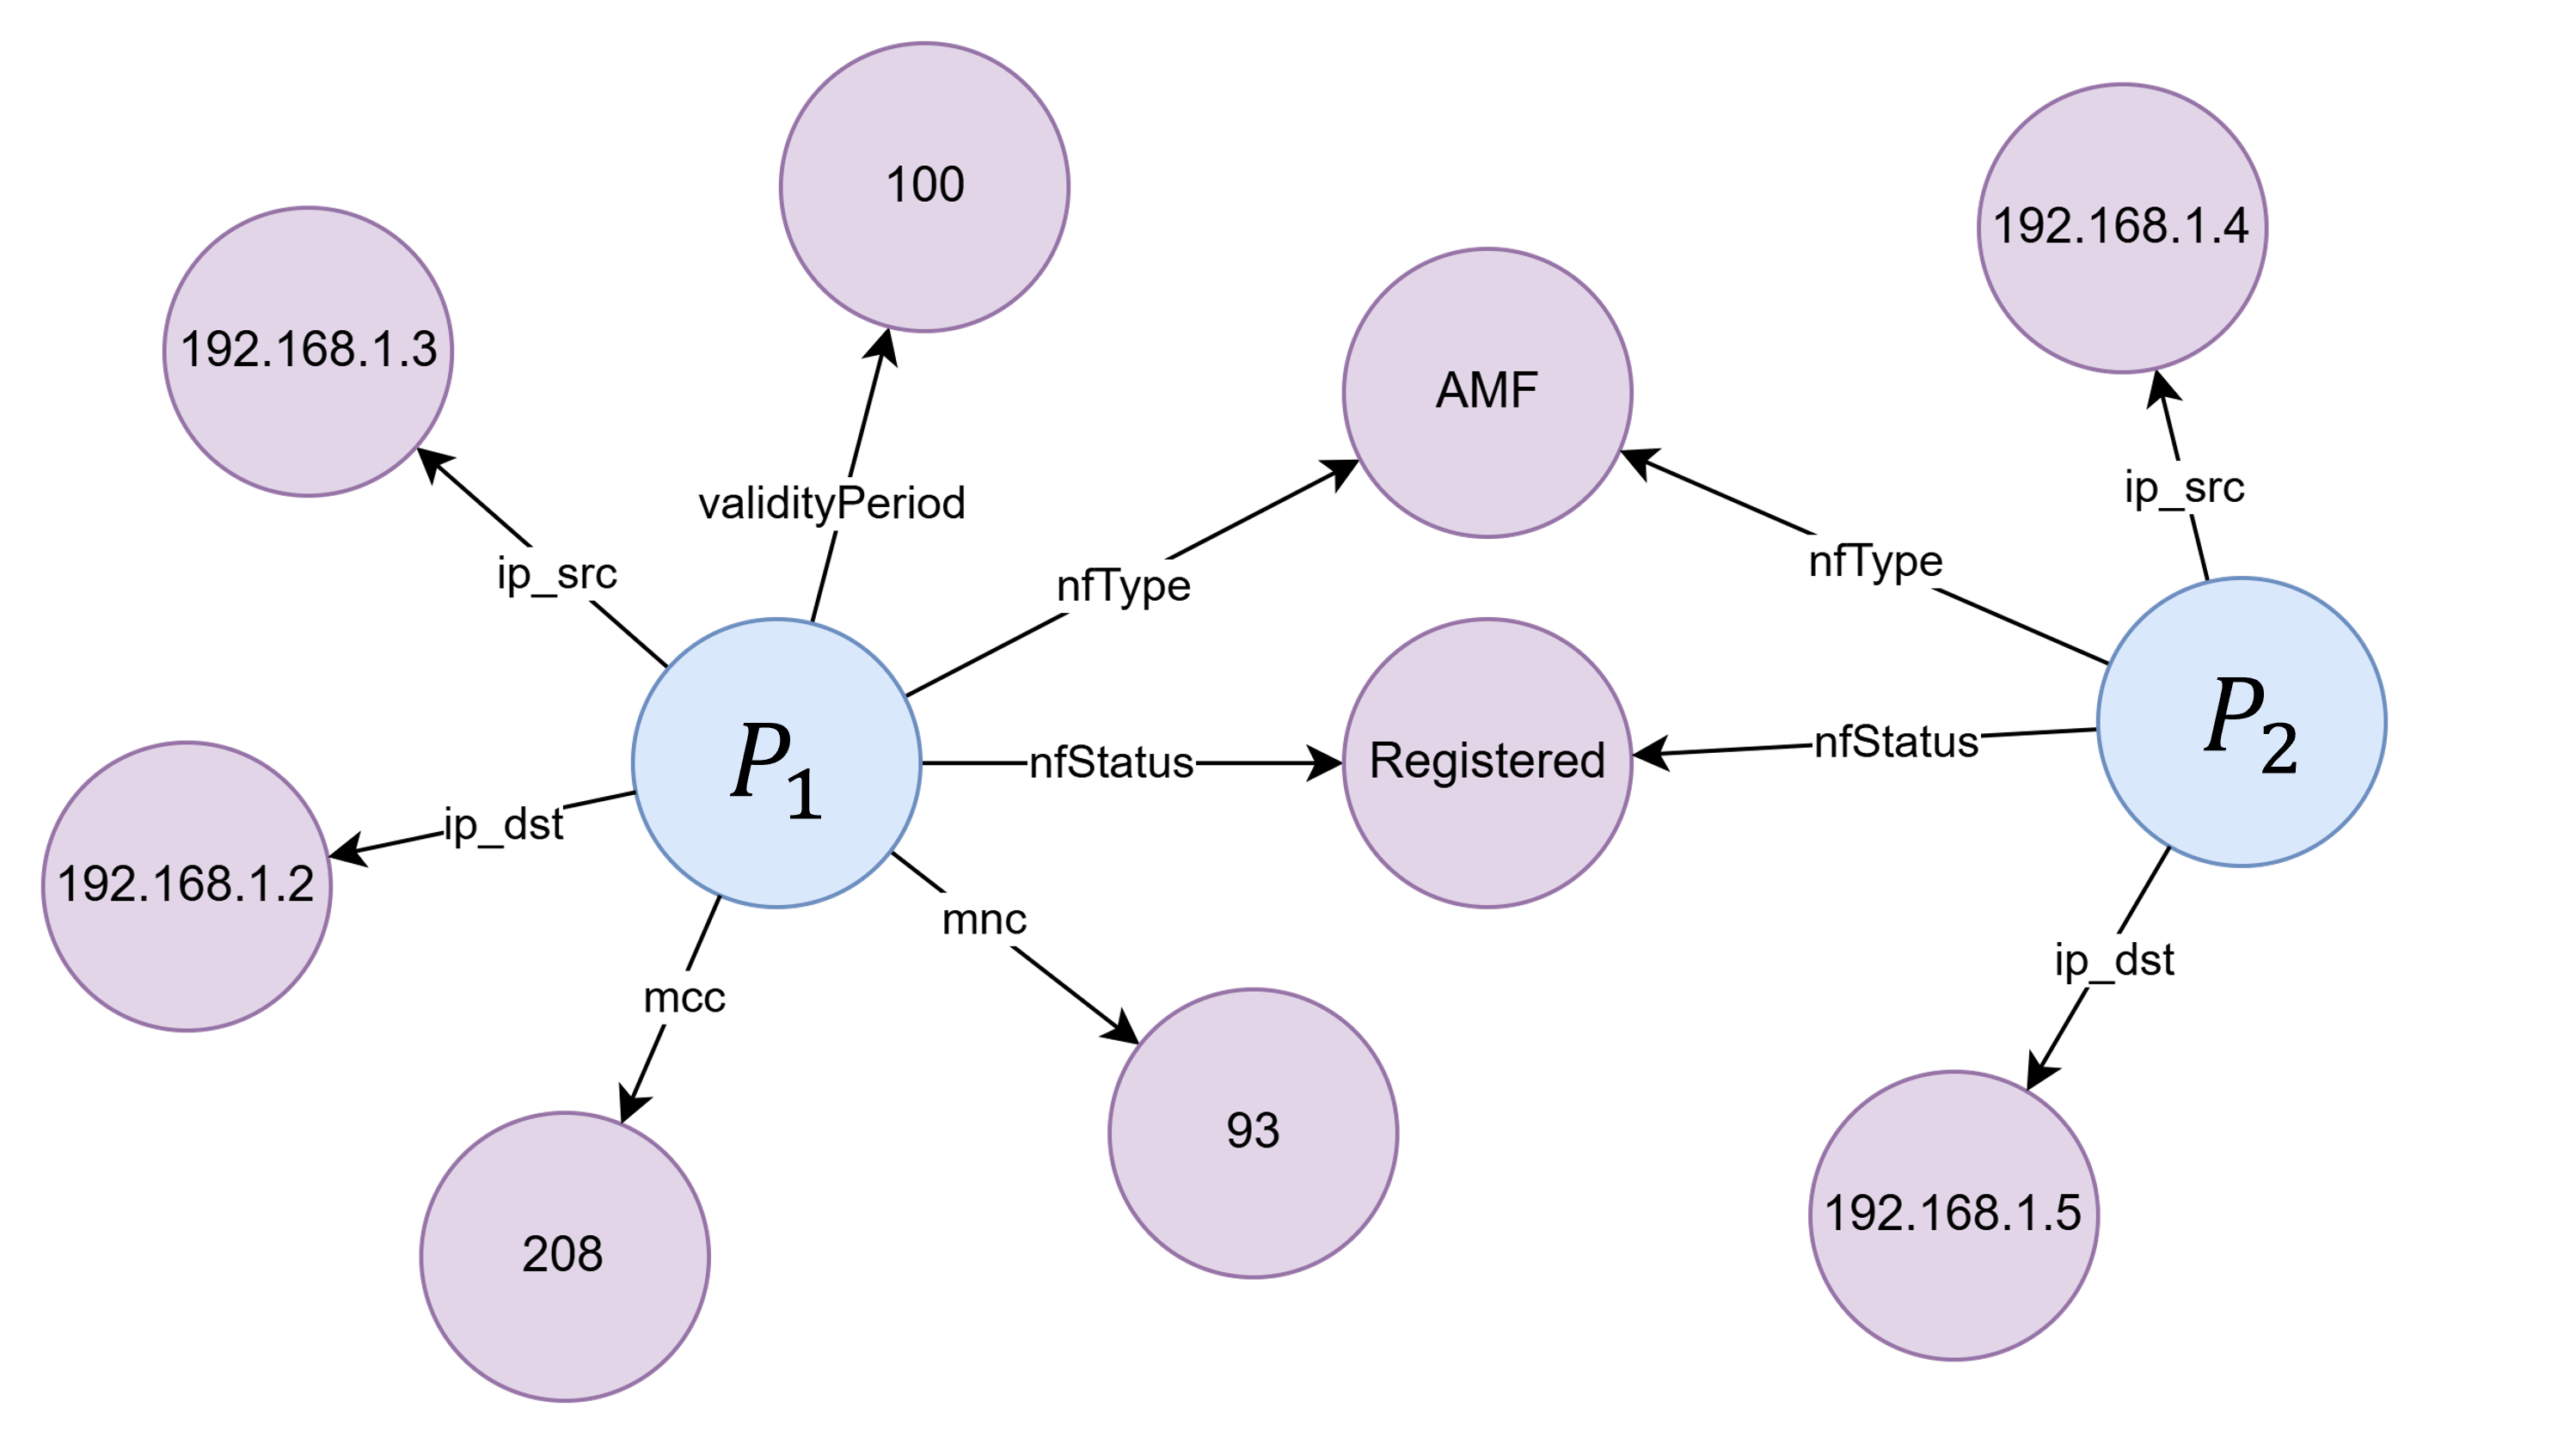
\includegraphics[width=0.7\linewidth]{figures/chapter3/graph_example.png}
\caption{Exemple de transformation de paquets en sous-graphes. Les nœuds mauves représentent les valeurs des paramètres, tandis que les nœuds bleus représentent les paquets eux-mêmes.}
\label{fig:graph_example}
\end{figure}

À la réception d’un paquet, au lieu de le représenter comme une arête entre deux entités, nous le modélisons sous forme de sous-graphe, où chaque paramètre est encodé comme un nœud indépendant relié à un nœud central qui représente le paquet. Chaque nœud de feature contient la valeur du champ associé, tandis que l’arête reliant ce nœud au paquet porte le nom du paramètre correspondant. À chaque nouveau paquet observé, un sous-graphe est créé. Pour chaque paramètre, un nouveau nœud est ajouté s’il n’a pas encore été rencontré. Dans le cas contraire, le nœud existant est réutilisé. Ce mécanisme permet de relier progressivement les différents sous-graphes entre eux à travers les paramètres partagés. La figure \ref{fig:graph_example} illustre le processus de transformation de deux paquets en deux sous graphes. Ces deux paquets partagent certains paramètres ayant des valeurs communes et leurs sous-graphes respectifs se retrouvent donc connectés. Comme il n’existe pas d’arcs reliant des nœuds de type paramètre entre eux, ni de nœuds centraux entre eux, on obtient ainsi un graphe biparti. Une autre caractéristique de notre graphe est qu’il est purement additif : la réception d’un paquet ne peut entraîner que l’ajout de nouveaux nœuds et d’arêtes, sans jamais modifier ni supprimer ceux déjà présents.

Cette décomposition permet de connecter des attributs issus de paquets différents en s’appuyant sur des caractéristiques communes, plutôt que sur la seule structure source–destination. Une telle représentation offre un niveau de granularité très fin et permet de capturer des interactions plus riches entre les caractéristiques des paquets. De plus, cette approche permet également d’identifier précisément les paramètres à l’origine d’un comportement anormal et se révèle donc, par construction, hautement interprétable.

Nous allons maintenant voir à quoi ressemblent les anomalies de chaque dimension une fois transformées en graphe.

\subsubsection{Anomalies sémantiques}

\begin{figure}[h]
\centering
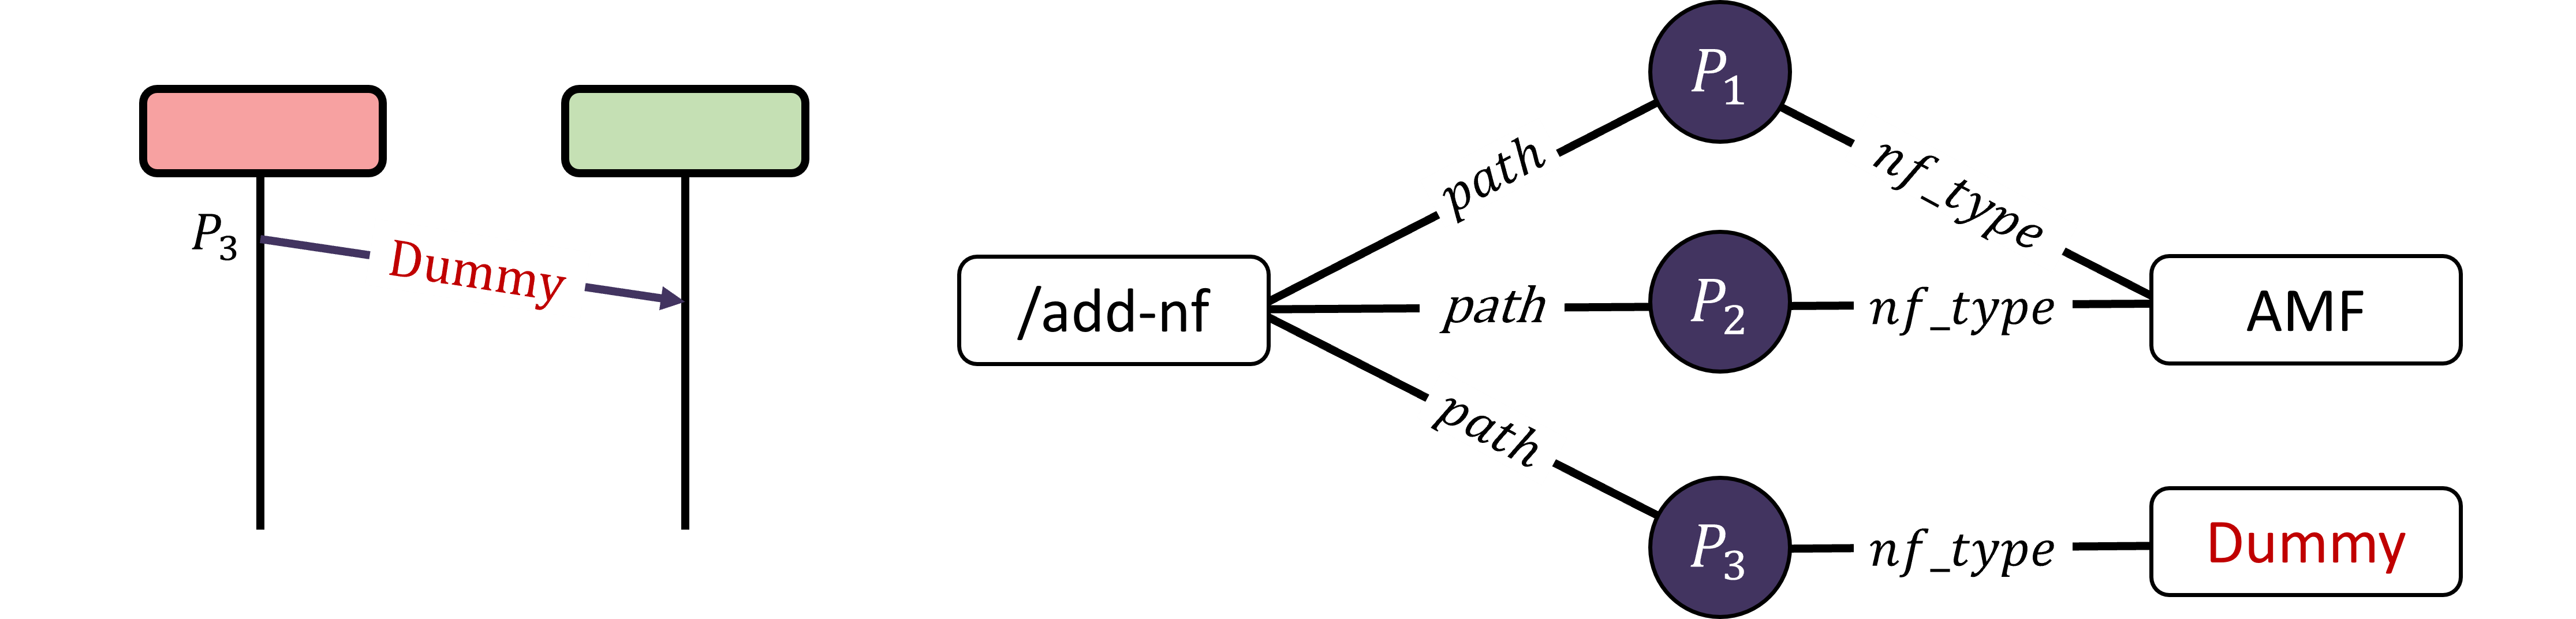
\includegraphics[width=\linewidth]{figures/chapter3/graph_semantique.png}
\caption{Anomalie sémantique et sa représentation sous forme de graphe}
\label{fig:graph_semantic}
\end{figure}

La figure \ref{fig:graph_semantic} illustre une anomalie sémantique dans laquelle un champ inhabituel apparaît. Dans le cas présent, il s’agit du paquet P3 qui contient la valeur \textit{NF Type} qui n'existe pas en 5G. Cette anomalie peut être détectée en le comparant aux autres paquets de même nature. On observe par exemple que les paquets P1 et P2, qui sont, comme P3, des requêtes vers l’endpoint \textit{add-nf}, possèdent des valeurs identiques pour le champ \textit{nf-type}, alors que P3 s’en écarte. Un modèle de détection ayant appris la structure usuelle de ce type de paquet pourrait ainsi identifier l’anomalie en observant uniquement le sous-graphe associé à P3.

\subsubsection{Anomalies topologiques}

\begin{figure}[h]
\centering
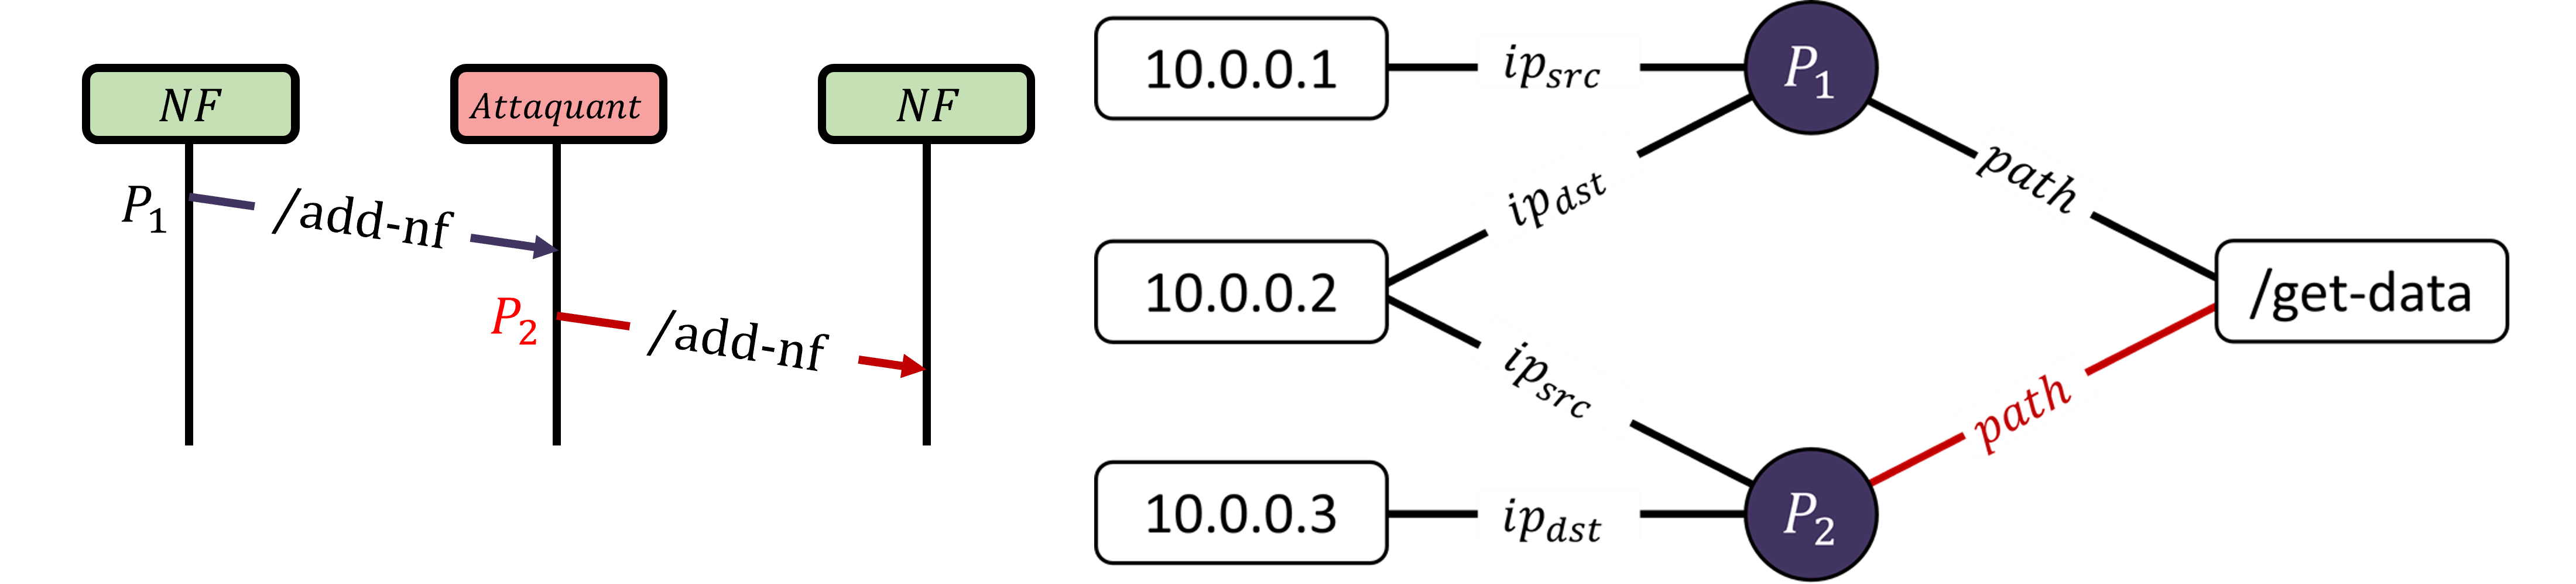
\includegraphics[width=\linewidth]{figures/chapter3/graph_topologique.png}
\caption{Anomalie topologique et sa représentation sous forme de graphe}
\label{fig:graph_topological}
\end{figure}

Sur la figure \ref{fig:graph_topological}, on observe un exemple d’attaque de type man-in-the-middle, où un paquet P1, initialement envoyé à l’adresse \textit{10.0.0.2}, génère l’envoi d’un nouveau paquet P2 identique (ici simplifié par le fait qu’il s’agisse du même endpoint), avec comme source la destination du paquet précédent et comme destination une nouvelle adresse. Ce cas ne peut normalement pas survenir en 5G, car il n’existe aucun scénario légitime de redirection de trafic de ce type. Le paquet P2 est une copie de P1 et paraît donc légitime pris individuellement. Il est nécessaire de prendre en compte le contexte de redirection afin de détecter l’anomalie.

\subsubsection{Anomalies séquentielles}

\begin{figure}[h]
\centering
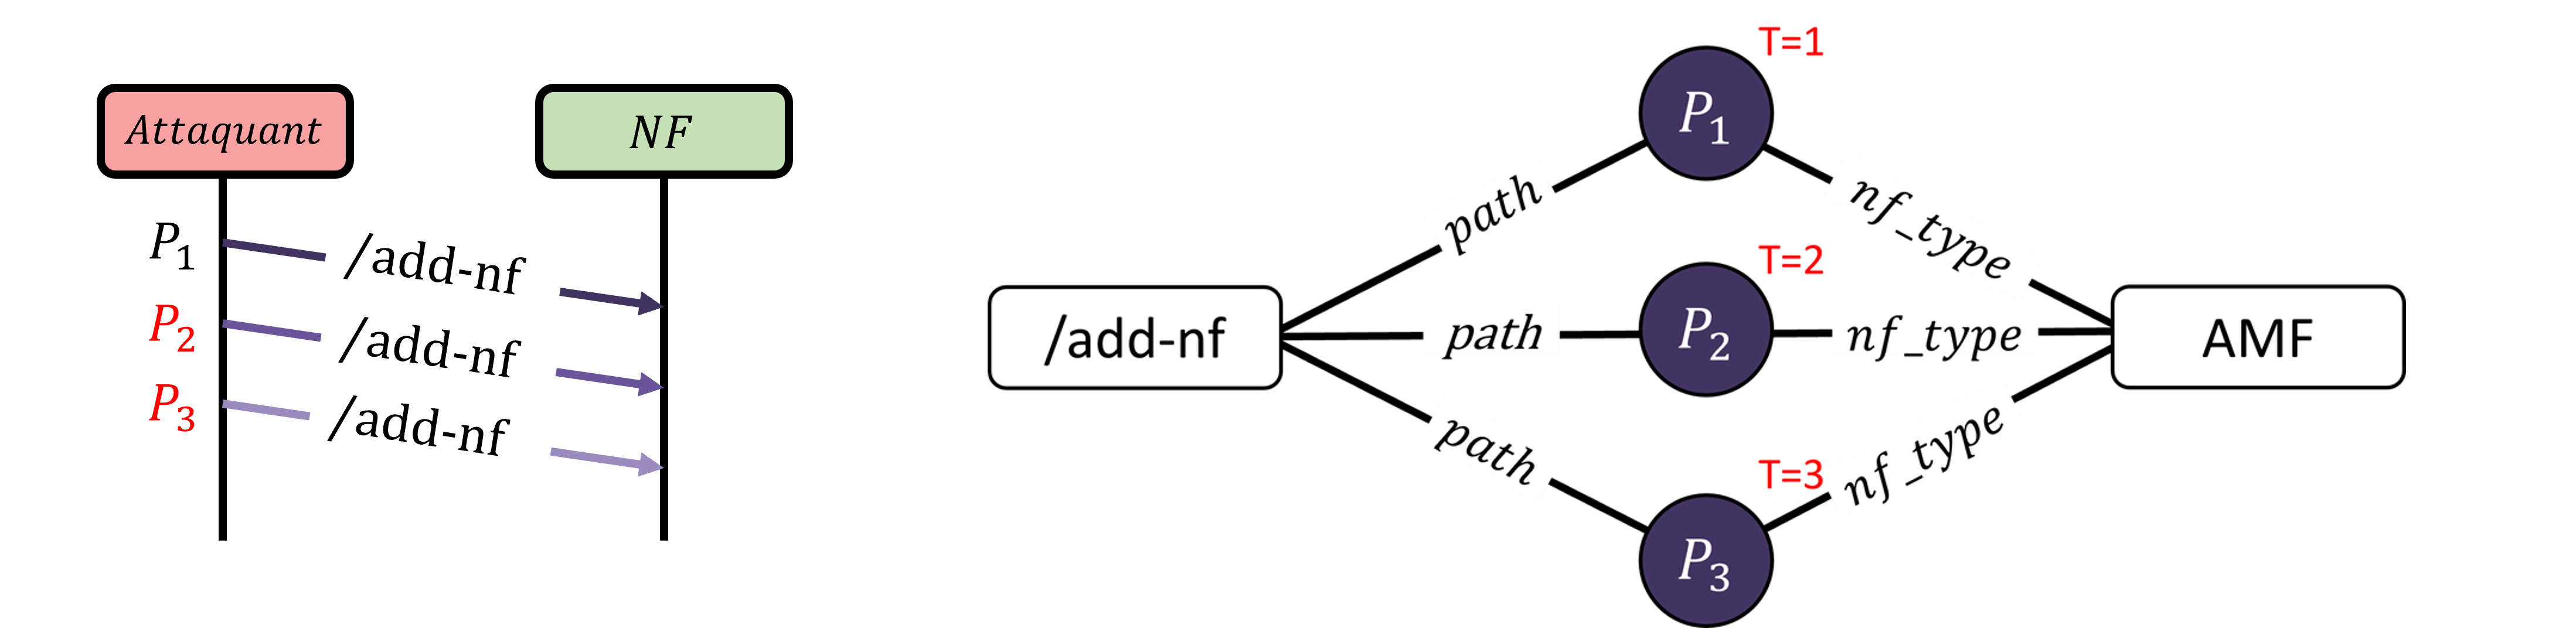
\includegraphics[width=\linewidth]{figures/chapter3/graph_seq.png}
\caption{Anomalie séquentielle et sa représentation sous forme de graphe}
\label{fig:graph_sequential}
\end{figure}

Enfin, sur la figure \ref{fig:graph_sequential}, on observe un exemple d’anomalie séquentielle. Dans ce cas, le contenu et les interactions des paquets sont normaux et la caractéristique anormale concerne uniquement leur ordre d'arrivée. Le problème est que le formalisme actuel ne modélise pas explicitement la dimension temporelle. Il serait possible de l’intégrer en ajoutant à chaque sous-graphe un nœud représentant le temps d’observation du paquet, mais avec cette approche la dimension temporelle serait confondue avec les autres paramètres, alors qu’elle est de nature distincte et particulièrement importante. Il est donc nécessaire de proposer une modélisation permettant d’intégrer le temps de manière plus explicite. Pour cela, nous nous intéressons aux graphes dynamiques, qui intègrent nativement la dimension temporelle, et que nous présentons dans les sections suivantes.

\section{Détection d’anomalies dans des graphs}

\subsection{Introduction aux GNN}

\begin{figure}[h]
\centering

\begin{minipage}{0.32\linewidth}
    \centering
    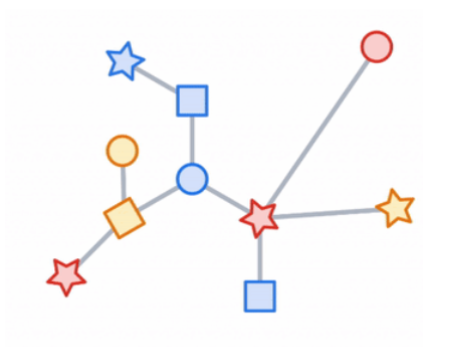
\includegraphics[width=\linewidth]{figures/chapter3/conv_1.png}
\end{minipage}
\hfill
\begin{minipage}{0.32\linewidth}
    \centering
    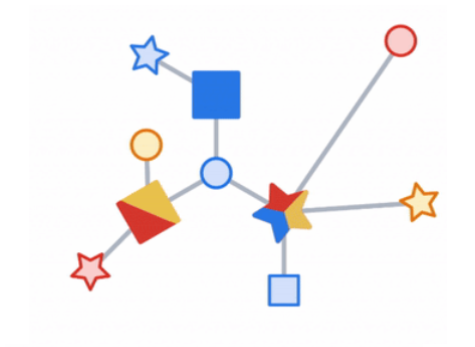
\includegraphics[width=\linewidth]{figures/chapter3/conv_2.png}
\end{minipage}
\hfill
\begin{minipage}{0.32\linewidth}
    \centering
    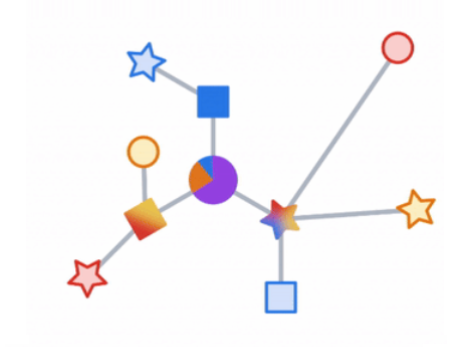
\includegraphics[width=\linewidth]{figures/chapter3/conv_3.png}
\end{minipage}

\caption{Illustration du processus de convolution. La première figure représente le graphe à son état initial. Dans la deuxième, une convolution est appliquée : on observe que les informations des nœuds feuilles sont agrégées et propagées à leurs voisins directs. Dans la troisième, une deuxième convolution est réalisée, et les informations précédemment propagées sont à nouveau diffusées jusqu’au nœud central du graphe, qui contient ainsi une représentation de son voisinage complet à distance 2.}
\label{fig:convolution}
\end{figure}

De manière générale, les graph neural networks sont très proches des CNN présentés précédemment. La principale différence est que les CNN opèrent sur des images, tandis que les GNN travaillent directement sur des graphes. Dans les deux cas, le principe repose sur une agrégation locale de l’information. Dans une image, cette agrégation s’effectue sur des voisinages de pixels, tandis que dans un graphe elle s’applique au voisinage des nœuds. Certains travaux proposent notamment de considérer une image comme un graphe de pixels et d’y appliquer des GNN, mais il s’agit d’une approche relativement marginale \cite{gnn_image}. L’idée fondamentale de ces deux types de modèles est que chaque itération du processus de convolution permet de diffuser l’information aux voisins directs. En procédant de manière récursive, chaque couche de convolution propage cette information à une distance croissante, augmentant progressivement le champ de réception des représentations. La figure \ref{fig:convolution} illustre ce processus de diffusion de l’information à travers réalisé par deux convolutions successives.

\subsection{Etat de l'art des GNN}
Le domaine des GNN est relativement récent et s’est fortement développé au cours de la dernière décennie. Le concept de réseaux de neurones sur graphes a été formellement introduit pour la première fois en 2008 par Scarselli et al.~\cite{gnn}, qui ont proposé un cadre neuronal pour l’apprentissage sur des données structurées en graphe, basé sur des mécanismes itératifs de propagation et d’agrégation d’états. Des travaux ultérieurs ont considérablement amélioré la praticabilité et la scalabilité de cette formulation initiale. En particulier, Kipf et Welling~\cite{gcn} ont introduit les Graph Convolutional Networks (GCN), qui simplifient le processus de propagation des messages en linéarisant l’agrégation de voisinage.

Dans leur formulation moderne, les GNN peuvent être vus comme réalisant des convolutions basées sur le voisinage, où l’information provenant des nœuds adjacents est agrégée afin d’enrichir la représentation de chaque nœud avec un contexte local. La plupart des architectures contemporaines de GNN suivent le paradigme de \textit{message passing} proposé par Gilmer et al.~\cite{mpnn}, composé de trois phases principales : la construction des messages à partir des embeddings des nœuds, l’agrégation des messages provenant des voisins, et la propagation (ou mise à jour) de l’information agrégée pour produire de nouvelles représentations des nœuds.

Sur la base du cadre MPNN standard, plusieurs extensions ont été proposées. Par exemple, les Graph Attention Networks (GAT)~\cite{gat} introduisent des mécanismes d’attention qui attribuent des poids adaptatifs aux nœuds voisins lors de l’agrégation. GraphSAGE~\cite{graphsage} permet un apprentissage inductif sur des nœuds jusqu’alors non vus en échantillonnant un voisinage de taille fixe et en appliquant des fonctions d’agrégation apprenables telles que la moyenne, le pooling ou des agrégateurs basés sur LSTM. D’autres variantes notables incluent les Graph Isomorphism Networks (GIN)~\cite{gin}, qui atteignent un pouvoir discriminant maximal parmi les GNN basés sur l’agrégation de voisinage.

Cependant, la plupart de ces architectures de GNN sont principalement conçues pour des graphes statiques. Or, nos données évoluent dans le temps et le graphe sous-jacent est dynamique. Nous nous intéressons donc aux modèles de graphes dynamiques, une classe encore plus récente de GNN. Parmi ces modèles, on distingue deux grandes catégories selon la granularité temporelle.

La première famille, les réseaux de graphes à temps discret (DTGN), constitue l’approche la plus directe pour intégrer l’information temporelle. Parmi les exemples notables de DTGN figurent EvolveGCN~\cite{evolvegcn} et T-GCN~\cite{tgcn}, qui appliquent des opérations GNN classiques sur des captures de l'état du graphe à intervalle régulier. Dans ce cas, la dimension temporelle est capturée de façon externe à l’aide de modèles récurrents utilisés en complément du GNN.

La seconde catégorie correspond aux réseaux de graphes en temps continu, qui opèrent à une granularité temporelle plus fine que les approches discrètes. Plutôt que de reposer sur des instantanés fixes, ces modèles traitent des séquences d’événements correspondant à l’ajout, la suppression ou la modification de nœuds et d’arêtes dans le graphe. Cette modélisation au niveau événementiel permet d’intégrer directement les dépendances temporelles dans le modèle, plutôt que de les traiter de manière externe. Un exemple emblématique de cette approche est le Temporal Graph Network (TGN)~\cite{tgn}, qui maintient des embeddings de nœuds évolutifs mis à jour en réponse aux événements entrants à l’aide d’une combinaison de mécanismes de message passing et de mémoire.

Une vue d’ensemble de l’apprentissage sur graphes dynamiques est proposée par Feng et al.~\cite{survey_gnn}, qui présentent une synthèse mettant en évidence les différences conceptuelles entre les modèles dynamiques à temps discret et à temps continu, ainsi qu’un benchmark étendu des principales méthodes de ces deux catégories.

\subsection{Formalismation adapté à l'utilisation de GNN dynamiques}
Pour considérer la dimension temporel et détecter les attaques de flood and multi-stage, il faut intégrer l'information temporel à notre détection et donc considérer les graphs dynamiques. On pourrait utiliser les graphs dynamiques discrets et c'est ce que fait d'ailleurs GSAD \cite{gsad}. Cette façon de gérer les graphes dynamiques est facile à comprendre et à implémenter, car les captures à intervalle régulier de l'état du graph forment une séquence de graphs indépendants sur lesquels on peut appliquer les GNN traditionnels sans modification majeure. Leur principal inconvénient est qu'ils sont très lourds et peu efficaces pour détecter les dépendances sur de longues périodes.

\begin{figure}[h]
\centering

% --- Première ligne ---
\begin{subfigure}{0.49\linewidth}
    \centering
    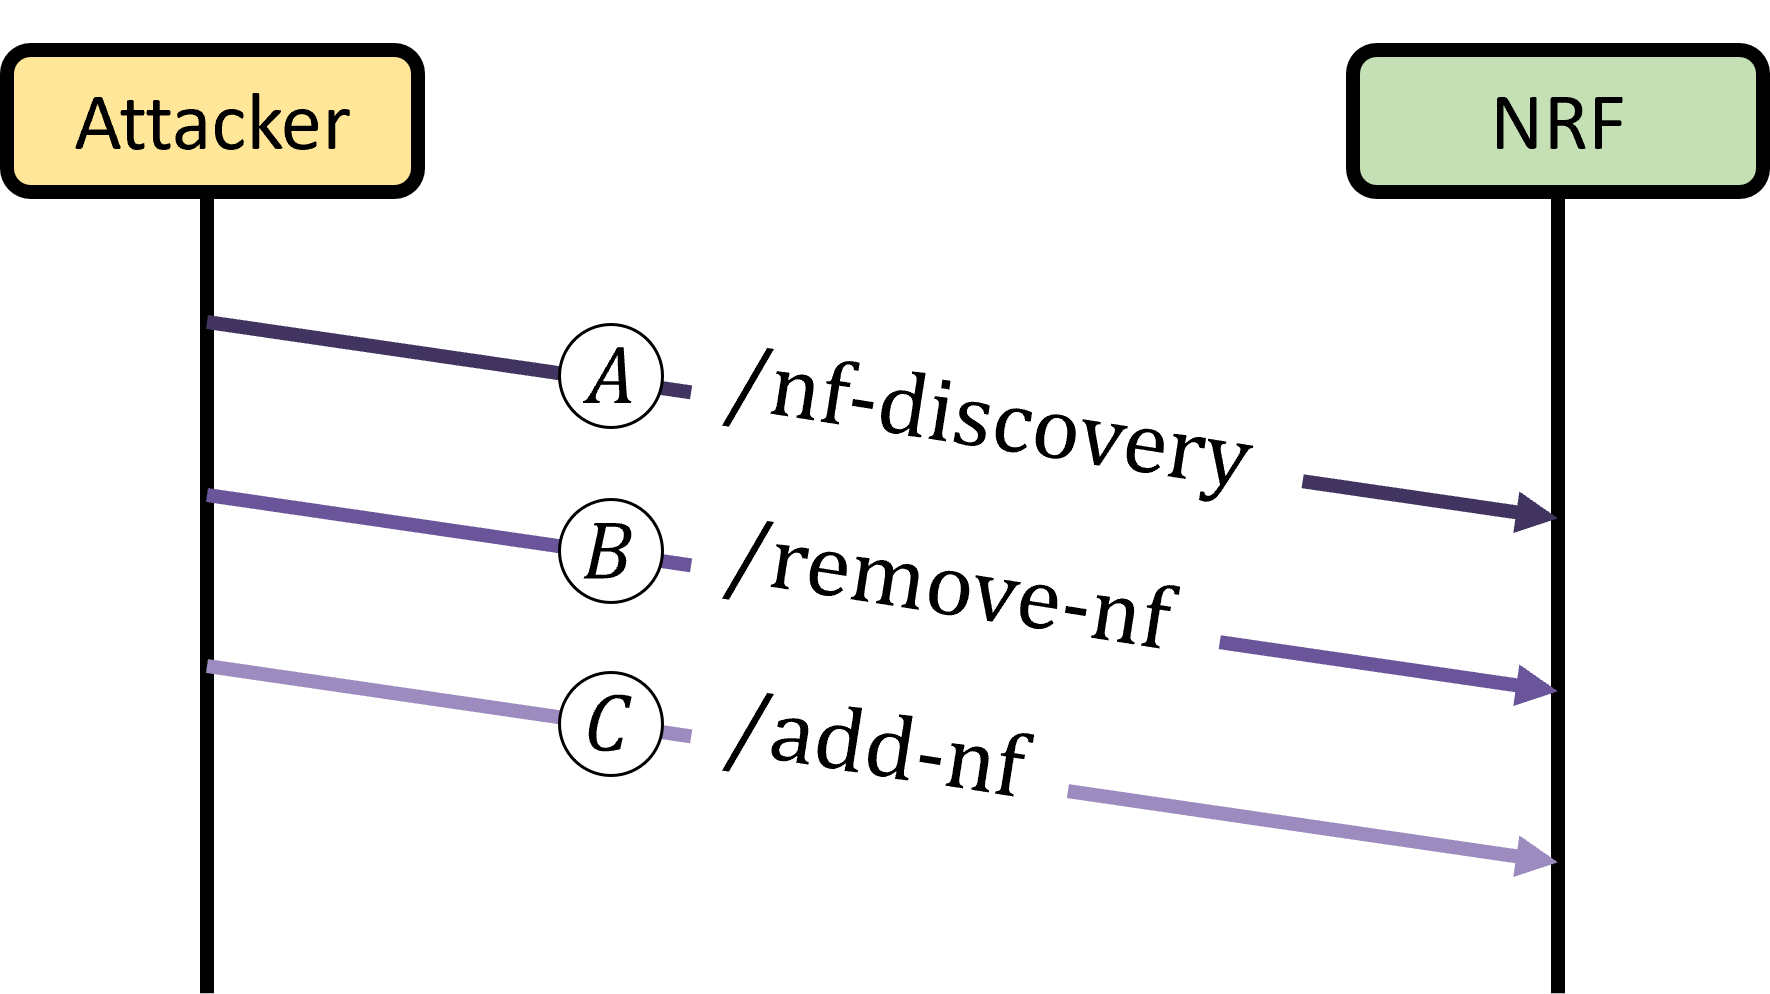
\includegraphics[width=\linewidth]{figures/chapter3/graph_continu_p1.png}
    \caption{Séquence d’envoi de trois paquets vers le NRF à des endpoints distincts.}
\end{subfigure}
\hfill
\begin{subfigure}{0.49\linewidth}
    \centering
    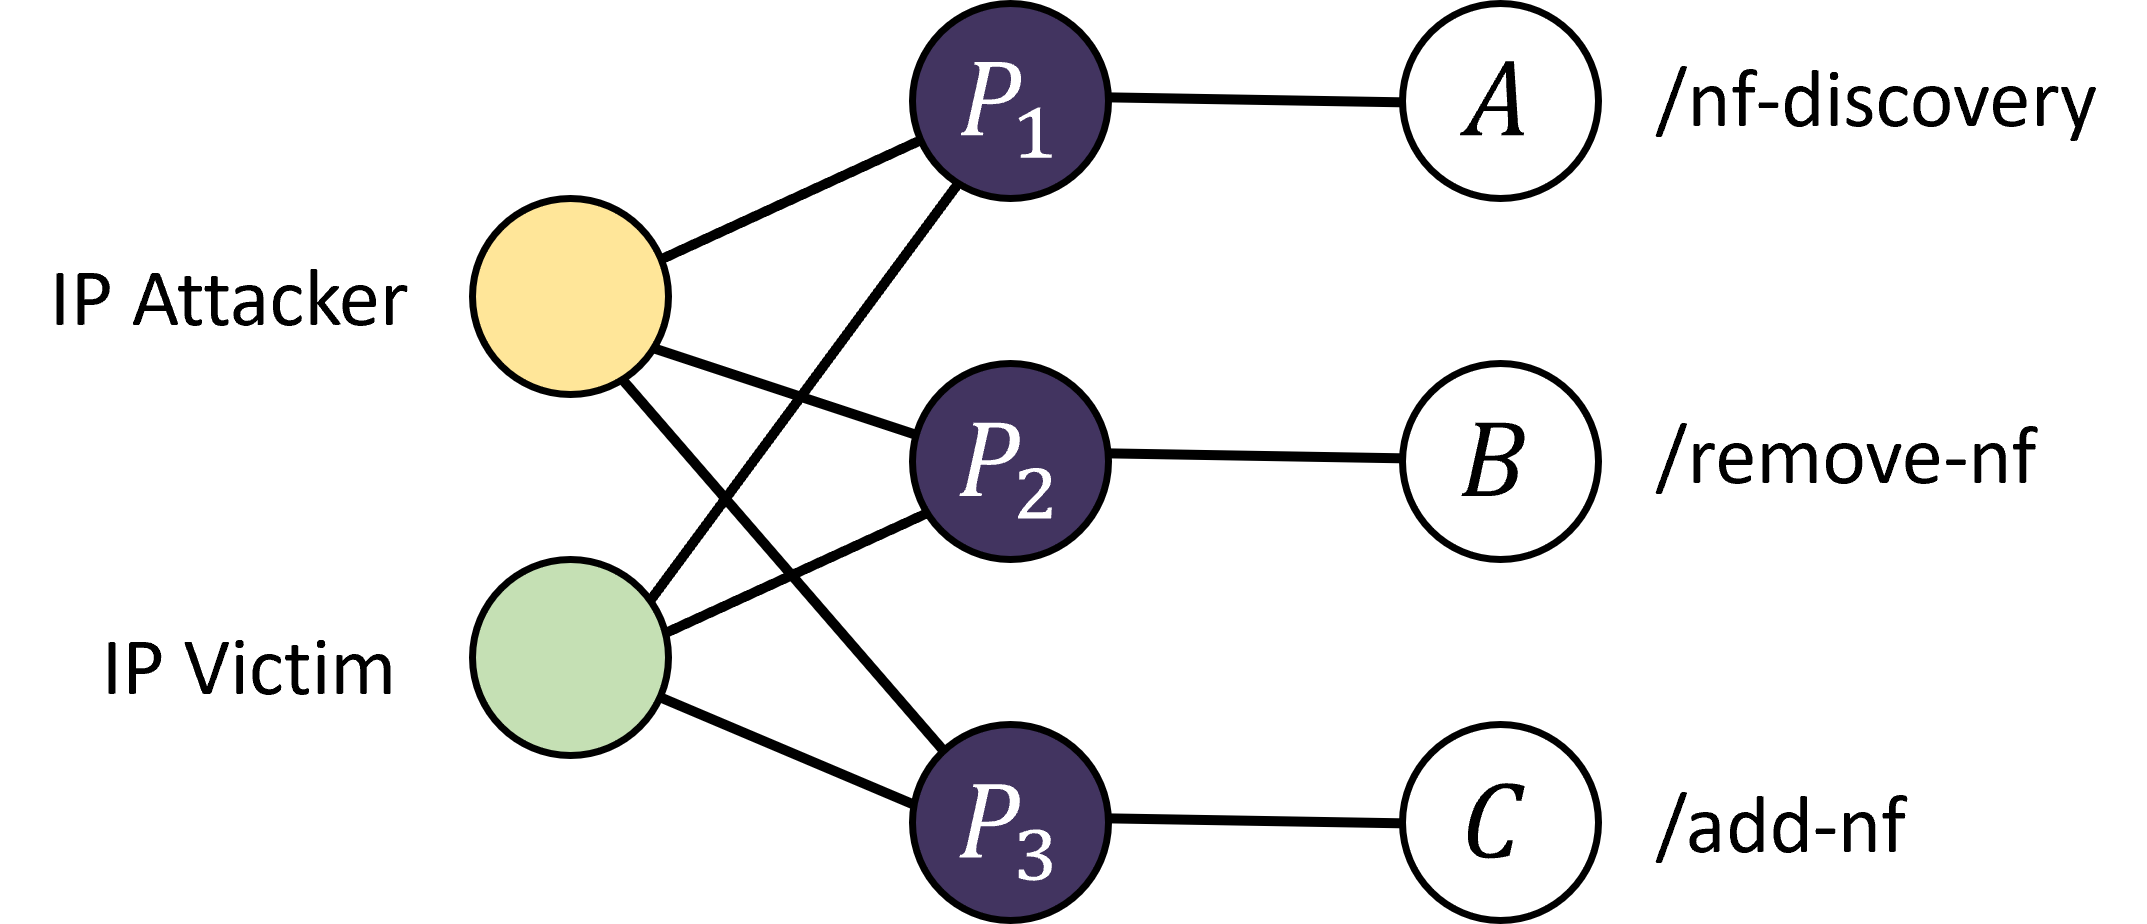
\includegraphics[width=\linewidth]{figures/chapter3/graph_continu_p2.png}
    \caption{Représentation sous forme de graphe statique. Chaque paquet génère un sous-graphe relié par des paramètres communs.}
\end{subfigure}

\vspace{0.5cm}

% --- Deuxième ligne ---
\begin{subfigure}{\linewidth}
    \centering
    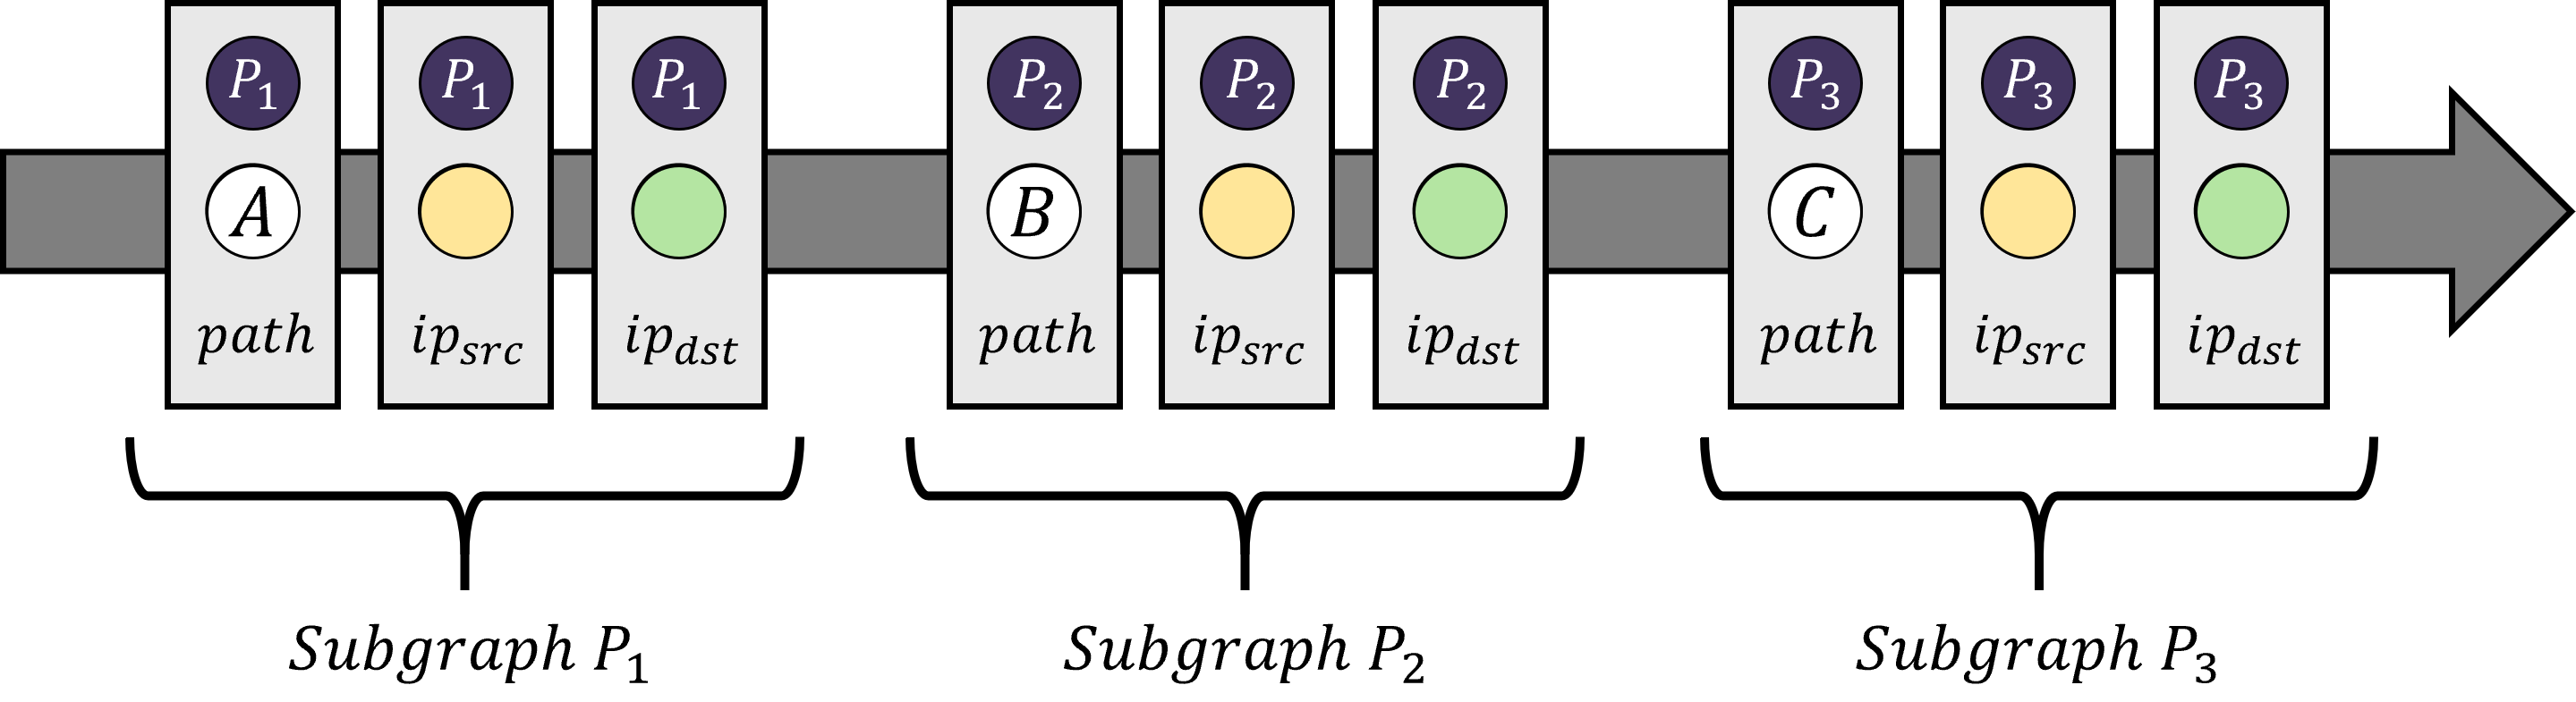
\includegraphics[width=\linewidth]{figures/chapter3/graph_continu_p3.png}
    \caption{Passage vers un graphe dynamique continu, où chaque arête est modélisée comme un événement contenant les informations des nœuds et arcs concernés.}
\end{subfigure}

\caption{Différentes représentations d’une même séquence d’échanges entre un attaquant et le NRF : diagramme de séquence, graphe statique, puis graphe dynamique continu.}
\label{fig:graph_continu}
\end{figure}

Nous nous intéressons donc davantage aux graphes dynamiques continus, tels qu’introduits dans le cadre de TGN~\cite{tgn}. Dans cette approche, plutôt que de représenter le graphe comme un objet statique décrivant un état à un instant donné, celui-ci est modélisé comme une séquence d’événements qui le construit progressivement.

\[
\mathcal{G} = \{ e_1, e_2, \dots, e_n \}
\]
où $e_i$ désigne l’événement apparaissant à la $i$-ème position dans la séquence.

Ces événements correspondent généralement à des ajouts, suppressions ou modifications de nœuds et d’arêtes. Toutefois, notre cadre est plus simple car notre graphe est purement additif. Chaque arête qui serait ajoutée dans un graphe traditionnel est représentée comme un événement défini par cette arête ainsi que par les deux nœuds qu’elle relie. 

\[
e_i = (u, v_i, x_i),
\]
où $u \in \mathcal{V}_c$ désigne un nœud central, $v_i \in \mathcal{V}_f$ un nœud de paramètre contenant la valeur de ce dernier et $\mathbf{z}_i \in \mathbb{R}^d$ le nom du paramètre contenu dans l’arête. 

Cette formulation nécessite d’adapter les algorithmes classiques utilisés dans les GNN, mais elle permet une représentation beaucoup plus fine, dans laquelle aucune information temporelle n’est perdue. La figure \ref{fig:graph_continu} illustre la transformation d'une forme de graphe statique à celle d'un graphe dynamique continu.

\subsection{Fonctionnement détaillé d'un GNN dynamique}
Pour comprendre le fonctionnement d’un GNN dynamique continu, nous allons nous appuyer sur le fonctionnement du Temporal Graph Network (TGN), l’un des modèles les plus populaires de cette catégorie. La plupart des GNN dynamiques suivent en effet une architecture globale très similaire, ce qui fait de TGN un exemple représentatif de la conception générale de cette famille de modèles. La figure \ref{fig:tgn} illustre l’architecture de TGN, qui se compose de quatre modules principaux : un module de mémoire, un module d’agrégation de messages, un module de mise à jour de la mémoire et un module d’inférence.

\begin{figure}[h]
\centering
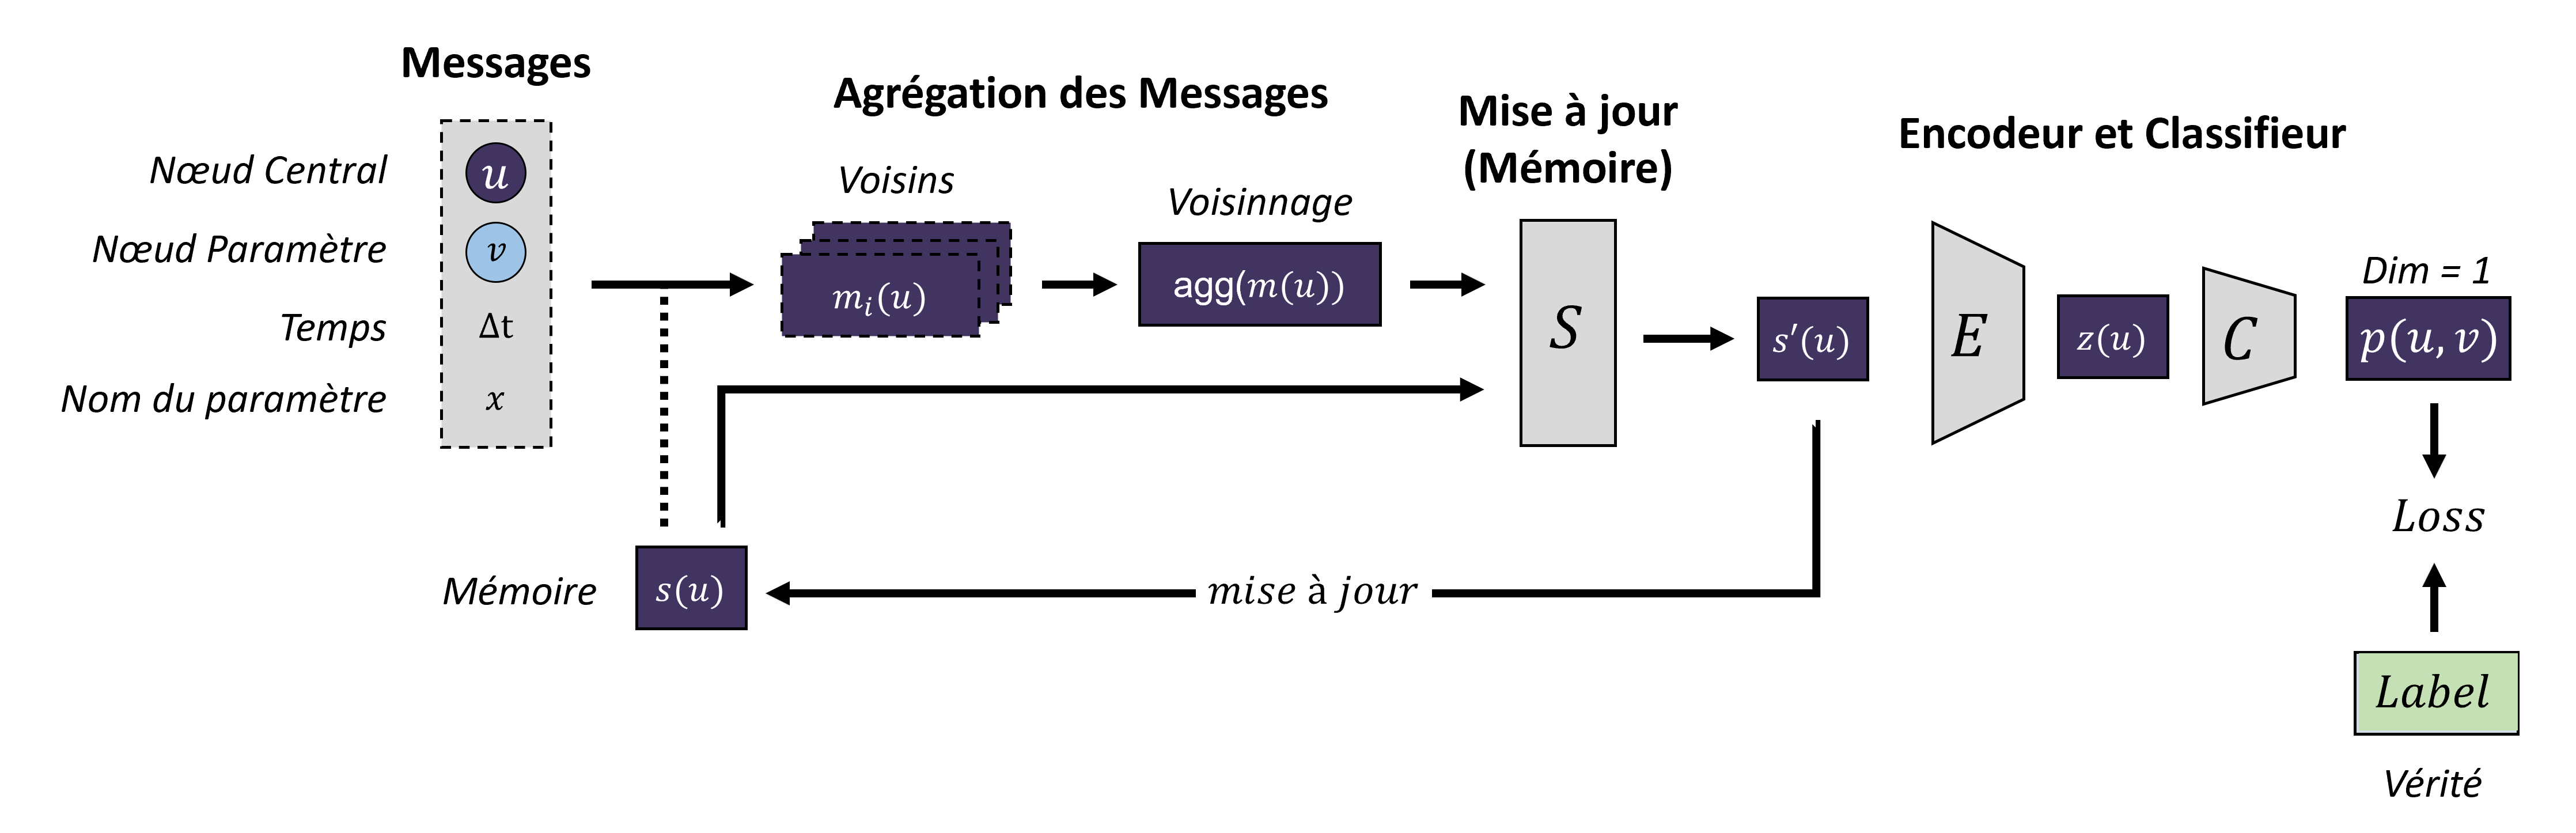
\includegraphics[width=\linewidth]{figures/chapter3/tgn.png}
\caption{Vue d'ensemble de l'architecture de TGN, illustrant les quatre modules principaux : mémoire, agrégation de messages, mise à jour de la mémoire et inférence.}
\label{fig:tgn}
\end{figure}

\subsubsection{Création des messages}
La première étape consiste à construire un message, c’est-à-dire un vecteur contenant l’ensemble des informations encodées associées à un événement du graphe dynamique. Dans un premier temps, les vecteurs associés aux nœuds centraux et aux nœuds paramètres sont initialisés comme des vecteurs nuls. Si ces nœuds ont déjà été impliqués dans des événements précédents, leurs représentations précédemment calculées est alors réutilisées. Le vecteur associé à l’arête est quant à lui déterminé à partir du nom du paramètre porté par l’événement. Dans notre cas, ce nom de paramètre correspond à un token textuel et il est donc nécessaire de l’encoder au préalable sous forme d’un vecteur numérique. La méthode utilisée pour cet encodage est présentée dans la section suivante.

\subsubsection{Agrégation des messages}
L’étape d’agrégation consiste à considérer l’ensemble des voisins du nœud source en cours de traitement, c’est-à-dire tous les événements dans lesquels ce nœud apparaît. On obtient ainsi une collection de messages qu'on d’agrége ensuite afin de produire un vecteur unique représentant le voisinage de distance 1 du nœud considéré. Cette agrégation peut être réalisée de différentes manières. TGN propose notamment plusieurs stratégies, parmi lesquelles l’utilisation de RNN, d’un mécanisme d’attention, une moyenne des messages ou bien de simplement conserver l’événement le plus récent.

\subsubsection{Mise à jour de la mémoire}
Afin de prendre en compte la dimension temporelle, le vecteur agrégé est combiné avec l’historique des représentations précédentes des éléments composant le message. Cet ensemble est ensuite transmis à un RNN, qui joue le rôle de module de mémoire apprenable. Ce module produit un nouveau vecteur représentant à la fois le message et son historique. Cette nouvelle représentation est utilisée pour les modules futurs et remplace également l’ancienne valeur stockée en mémoire. TGN propose notamment d’utiliser des architectures de type LSTM ou GRU pour implémenter ce module de mémoire.

\subsubsection{Encodeur et Classifieur}
% l'encodeur est le modèle qui va perform the convolution et retrieve the node’s neighborhood up to N hops correspondant au nombre N de convolution and pass it through an encoder (here, a multi-head attention mechanism) which outputs a vector representing this extended neighborhood.


\subsection{Adaptation des algorithmes à notre cas d'utilisation}
% nous on a pas besoin de l'information temporel donc on la dégage


%\subsection{Prise en compte des arcs}

\section{Encodage des paramètres de dimension non-fini}
% si on veut pouvoir considérer tous les paramètres possibles d'un paquet on se retrouve avec un nombre gigantesque de features. Plus ce nombre de feature est grand plus ça va ralentir l'apprentissage ET si on a pas implémenté une feature on a moins de messages possible et donc de features donc ce nombre de feature n'est pas non plus constant entre les implémentations et leurs versions. 
% y'a aussi beaucoup de redondance entre features par exemple entre ... mais aussi des nuances sémantiques comme .. 
% ces features doivent etre encodées pour être traiter par des modèles d'apprentissage profond et si on 


% ce qui serait bien ça serait donc de pouvoir traiter une quantité indénombrable de features et de ne pas se limiter à un nombre fini de features préalablement définies.
% on a aussi un autre problème notamment avec 
% (Hétérogénéité d’opérateur = différents vocabulaire → nombre de variable indénombrable)

% We could encode each parameter name as orthogonal vectors mais y'a 2 problèmes si on le fait directement sur nos données actuelles, Premièrement la valeur des features qu'on a n'est pas homogène. Ainsi comme on se retrouve vite avec beaucoup 

% ensuite on a beaucoup de redondance entre certains paramètres par exemple IMSI et SUCI qui sont deux formats différents d'un même identifiant utilisateur, ces redondances on augmente d'autant plus l'espace que prennent . 

% Le problème c'est qu'on a un nombre indénombrable de paramètres potentiels, premièrement à cause de l'utilisation d'appels d'API car un attaquant peut injecter des paquets contenants des paramètres arbitraires qu'il faut tout de même encoder.

% le nombre de noms de paramètres potentiellement observables dans le trafic 5G est extrêmement important, pouvant atteindre plusieurs centaines de milliers de features distinctes. Une approche naïve consisterait à représenter chaque paramètre par un vecteur orthogonal (\textit{one-hot encoding}), mais cela conduirait à des représentations de très grande dimension, peu efficaces en pratique.

% De plus, une telle représentation ne permettrait pas de capturer les similarités sémantiques entre paramètres. Or, il est souhaitable que des paramètres conceptuellement proches, comme \textit{source-ip} et \textit{destination-ip}, possèdent des représentations relativement similaires dans l’espace latent. Pour cette raison, il est préférable d’utiliser des embeddings appris, capables de projeter les paramètres dans un espace vectoriel dense de dimension réduite tout en préservant certaines relations sémantiques.

\subsection{Sélection et encodage des features}
% Le fait de conserver dans le graph toutes les features extraites soulève tout de même plusieurs problématiques. Tout d’abord, le nombre de features extraites est particulièrement élevé. Dans nos données, un paquet contient en moyenne 18 features, ce qui représente déjà une quantité importante d’information à traiter. De plus, dans les données générées, certains paquets peuvent ainsi contenir jusqu’à 200 features différentes ce qui augmente significativement la complexité des graphes générés.


% Le deuxième problème est que parmi tout ce vocabulaire très riche y a beaucoup de paramètres qui ont une très forte corrélation sémantique. On se retrouve au final avec des paramètres  comme les IMSI et le SUCI qui désignent la même chose sur des formats différents. De fait, dans nos paramètres y'en a beaucoup qu'on pourrait regrouper et ainsi réduire la complexité de nos graphs

% Le truc c'est qu'au final dans ces paramètres ils ont pas toutes les mêmes importances pour la détection. Par exemple l'endpoint d'api à beaucoup plus d'impact que le débit de transmission. 

% Deep packet analysis requires parsing packets in order to extract attributes from the application layers. The IP layer is used to identify communicating entities. For each application layer, we search for a predefined set of 20 attributes. These attributes only represent a fraction of the existing ones as many of the other ones are redundant or carry limited security-relevant information. Moreover, increasing the number of features can hinder the learning process by introducing noise and increasing model complexity. The selected features are chosen to be directly aligned with the considered threat model, as they capture protocol fields and interaction attributes that are explicitly exploited or manipulated by known attacks. Among these features, we consider for instance the method and path api calls, session identifiers for PFCP, as well as the nested IP addresses carried by the intermediate IP layer encapsulated within GTP. Moreover, this feature set can be easily extended by a human operator at deployment time, based on their expertise, either by adding generally suspicious features or by incorporating features corresponding to entirely novel attack patterns. The complete list of selected features is available in our GitHub repository \cite{anomaly_detect}.

% In order to be processed by deep learning models, they features need to be encoded. Since we currently have only a small number of features, a simple one-hot encoding is sufficient. However, if the number of features were to increase in the future, it could be worthwhile to explore Natural Language Processing (NLP) inspired encoding methods such as Glove\cite{glove} or BERT \cite{bert}. These methods generate embeddings such that semantically similar features are mapped to nearby vectors, which could facilitate faster convergence during the initial training epochs.

\subsection{Utilisation de Linegraph}
% Toujours dans l'optique de réduire la complexité de nos graphes, on peut aussi envisager d'utiliser des linegraph

\section{Conclusion}

\ifdefined\included
\else
\bibliographystyle{acm}
\bibliography{These}
\end{document}
\fi

\ifdefined\included
\else
\documentclass[a4paper,11pt,twoside]{StyleThese}
\include{formatAndDefs}
\sloppy
\begin{document}
\setcounter{chapter}{3} %% Numéro du chapitre précédent ;)
\dominitoc
\faketableofcontents
\fi

\chapter{From theory to practice: A more generalizable and applicable implementation with Open Source MANO}\label{chap:transition}
\minitoc

\section{Challenges in Adapting Theoretical Models to Existing Standards}
\subsection{Multi-cluster orchestration}
\subsection{Abstraction gaps: containerized vs. virtualized Resources}
\subsection{The overlooked role of energy in NFV orchestrators}

\section{CNF placement and migration with OSM}
\subsection{Architectural overview of our system}
\subsection{OSM as a NFV MANO orchestrator}
\subsection{Deploying CNFs: Kubernetes, Helm \& OSM Integration}
\subsection{Monitoring \& optimization}

\section{Experimental validation}
\subsection{Experimental setup}
\subsection{Service placement experiments}
\subsection{Service migration experiments}

\section{Conclusion}

\ifdefined\included
\else
\bibliographystyle{acm}
\bibliography{These}
\end{document}
\fi

\ifdefined\included
\else
\documentclass[a4paper,11pt,twoside]{StyleThese}
\include{formatAndDefs}
\sloppy
\begin{document}
\fi


\chapter*{Conclusion}
\addstarredchapter{Conclusion} %Sinon cela n'apparait pas dans la table des matières
Au cours de cette thèse, nous avons tâché d'étudier les évolutions introduites par la 5G, tant du point de vue des nouvelles surfaces d'attaque que de la nature des menaces auxquelles ces réseaux sont exposés. Cette analyse nous a permis de mettre en évidence que la notion d'attaque 5G demeure encore insuffisamment unifiée dans la littérature. Les travaux existants adoptent des définitions et des niveaux de réalisme très hétérogènes, rendant difficile la comparaison des approches proposées. Afin de répondre à cette limite, nous avons proposé une classification des attaques visant à fournir un cadre commun pour l'étude et l'évaluation des mécanismes de détection.

Nous avons également montré que les spécificités des réseaux 5G nécessitent une analyse approfondie des paquets échangés, en prenant simultanément en compte trois dimensions complémentaires : la dimension sémantique, la dimension séquentielle et la dimension topologique. Pour répondre à cette problématique, nous avons proposé un nouveau formalisme reposant sur les graphes dynamiques continus, capable de représenter conjointement ces trois aspects tout en offrant un niveau d'interprétabilité élevé, indispensable dans le contexte de la cybersécurité.

Par ailleurs, nos travaux ont mis en évidence le manque cruel de datasets publics, complets et reproductibles dans l'état de l'art pour évaluer les approches de détection dans des environnements 5G. Afin de pallier cette limitation, nous avons conçu notre propre dataset couvrant un ensemble étendu de procédures bénignes et de scénarios d'attaque, tout en veillant à garantir sa qualité et sa reproductibilité afin de faciliter la comparaison de futurs travaux.

Enfin, nous avons évalué plusieurs architectures de réseaux de neurones sur graphes dynamiques afin d'étudier leur capacité à exploiter le formalisme proposé. Les résultats obtenus montrent que cette représentation est adaptée à la détection d'anomalies dans les réseaux 5G, en particulier dans un cadre supervisé, où les meilleurs modèles atteignent une accuracy d'environ 94\%. Ces résultats confirment l'intérêt des graphes dynamiques pour représenter les interactions complexes observées dans les infrastructures 5G et ouvrent la voie à de futurs travaux visant à améliorer encore leurs performances ainsi que leur capacité de généralisation à des environnements opérationnels.

\section{Contributions}

Les principales contributions de cette thèse peuvent être résumées peuvent être résumées comme suit :

\begin{itemize}
\item \textbf{Analyse critique des attaques 5G et des cadres de catégorisation existants.} Nous mettons en évidence les limites des cadres de catégorisation existants et proposons une classification permettant de structurer les différentes familles d'attaques selon les surfaces du réseau 5G qu'elles ciblent.
\item \textbf{Proposition d'un formalisme de graphes dynamiques continus.} Nous introduisons une représentation permettant de capturer simultanément les dimensions sémantique, temporelle et topologique des échanges au sein d'un réseau 5G, tout en conservant un haut niveau d'interprétabilité.
\item \textbf{Conception d'un dataset de trafic de contrôle 5G.} Nous proposons un nouveau dataset couvrant un ensemble étendu de procédures bénignes et de scénarios d'attaque, afin de pallier le manque de jeux de données publics représentatifs des environnements 5G.
\item \textbf{Evaluation comparative de modèles de détection d'anomalies} Nous comparons plusieurs architectures de l'état de l'art, dans des contextes supervisés et non supervisés, afin d'évaluer leur aptitude à exploiter le formalisme proposé pour la détection d'anomalies dans les réseaux 5G.
\end{itemize}


\section{Limites et perspectives}
Bien que les principaux objectifs de cette thèse aient été atteints, plusieurs pistes d'amélioration et d'extension n'ont pas pu être explorées pleinement et pourront faire l'objet de travaux futurs.

\subsection{Optimisation de l'implémentation et utilisation de BERT}
Une perspective concerne l'optimisation de l'implémentation utilisée pour l'évaluation des modèles. Nous avions initialement prévu d'intégrer des modèles d'encodage plus complexes, tel que BERT, afin d'étudier leur impact sur les performances. Cependant, l'implémentation actuelle de DyGLib présente plusieurs limitations en termes d'efficacité computationnelle, rendant l'entraînement de modèles plus coûteux difficilement envisageable.

En particulier, la gestion mémoire adoptée par la librairie n'est pas totalement adaptée aux contraintes des graphes dynamiques. L'espace mémoire est réservé pour des nœuds futurs avant leur apparition, et aucun mécanisme efficace de suppression des nœuds trop anciens n'est proposé. Cela conduit progressivement à une augmentation importante de la taille du graphe et ralentit fortement les entraînements.

Ces contraintes nous ont conduits à ne pas intégrer BERT dans les expérimentations finales, malgré son potentiel pour améliorer la représentation sémantique des paramètres réseau. Une optimisation de l'implémentation permettrait ainsi d'explorer ces modèles plus complexes dans de futurs travaux.

\subsection{Mise en place d'un modèle spécialisé}
Dans cette étude, nous avons principalement utilisé des modèles issus de l'état de l'art afin d'évaluer notre formalisme, avec seulement quelques adaptations mineures. Toutefois, ces architectures ne sont pas nécessairement optimisées pour répondre aux spécificités de notre problématique.

Une perspective d'amélioration serait donc de concevoir une architecture dédiée, comme cela est fréquemment réalisé dans les travaux existants. Dans notre cas, une telle architecture pourrait notamment exploiter les particularités de notre représentation sous forme de graphe biparti, ainsi que le fait que l'information pertinente soit portée par les arcs plutôt que par les nœuds. Cette approche permettrait potentiellement d'obtenir un modèle mieux adapté à la structure des données et aux objectifs de détection considérés.

\subsection{Extension du dataset CTD5G}
Le dataset CTD5G couvre de manière satisfaisante les surfaces d'attaque définies dans le périmètre de cette étude et permet de détecter les attaques qui leur sont associées. Néanmoins, certaines surfaces n'ont pas pu être prises en compte.

C'est notamment le cas de l'AN, pour lequel le dataset contient du trafic légitime mais aucun scénario d'attaque. Les procédures de \textit{handover} constituent également une piste d'extension, puisqu'elles mettent en jeu une pile protocolaire spécifique ainsi que des scénarios impliquant le changement de gNB par un UE au cours de son déplacement.

Le \textit{slicing} représente une autre perspective intéressante. Plusieurs attaques ciblant ce mécanisme ont déjà été proposées dans la littérature \cite{slicing_attack}. Toutefois, les implémentations open source actuelles offrent un support encore limité de cette fonctionnalité. En pratique, l'identifiant de slice est principalement utilisé comme un simple critère de filtrage, plutôt que comme un véritable mécanisme d'isolation logique entre les différentes tranches du réseau.

Bien que la couverture actuelle du dataset soit suffisante pour les surfaces d'attaque considérées dans le périmètre de cette étude, l'intégration de ces nouvelles surfaces permettrait d'améliorer davantage sa représentativité en regard des fonctionnalités avancées des réseaux 5G.

\subsection{Intégration d'informations système}
Les logs systèmes sont fréquemment utilisés pour la détection d'anomalies dans le domaine des systèmes distribués \cite{dist_log_trace}. Dans notre approche, nous avons choisi de ne pas les intégrer, car ils constituent une représentation indirecte et potentiellement partielle des événements réseau. 

Toutefois, plutôt que de s'appuyer sur la surcouche que constituent les logs, une approche alternative consisterait à surveiller directement les appels systèmes effectués par les machines hôtes afin d'intégrer des informations issues de l'environnement d'exécution. Ces données pourraient permettre d'identifier des comportements complémentaires, comme les phases d'une intrusion ainsi que les conséquences système des attaques réseau, telles que les surcharges ou les pertes de connectivité.

Le travail de Raulin et al. \cite{baguette} propose notamment une modélisation des appels systèmes sous forme de graphes, ce qui ouvre la possibilité d'adapter ce formalisme à notre représentation et de combiner les informations réseau et système. Une telle approche nécessiterait néanmoins une étape de sélection des événements pertinents afin d'écarter les comportements systèmes non liés à la détection d'attaques réseau, ce qui représente un défi supplémentaire mais constitue une perspective intéressante.

\section{Synthèse}
Au cours de cette thèse, nous avons étudié les approches existantes en détection d'anomalies dans les réseaux 5G et mis en évidence plusieurs limites de l'état de l'art, notamment concernant les attaques considérées, les datasets disponibles et les méthodes de détection proposées.

La principale contribution de ce travail est la proposition d'un nouveau formalisme permettant de répondre à ces limites. Celui-ci permet de détecter des attaques couvrant les trois dimensions étudiées, tout en conservant une forte capacité d'explicabilité. Cette propriété le rend particulièrement adapté aux environnements nécessitant une validation humaine, comme les SOC.

Les résultats obtenus sont encourageants, avec des performances atteignant jusqu'à 94\% d'accuracy. Ces performances pourraient encore être améliorées par des modèles plus spécialisés ou des étapes de \textit{fine-tuning}.

% Enfin, plusieurs extensions sont envisageables, notamment l'intégration d'informations issues de l'environnement système afin de compléter l'analyse basée sur les données réseau.

Ainsi, cette thèse ouvre de nouvelles perspectives pour l'amélioration des méthodes et outils existants, tout en proposant de nouvelles opportunités grâce au formalisme développé et à l'exploitation de modèles de graphes continus dynamiques.

\ifdefined\included
\else
\bibliographystyle{acm}
\bibliography{These}
\end{document}
\fi

\appendix

% \include{Annexe1}

\bibliographystyle{StyleThese}
%\bibliographystyle{plain}
\bibliography{These}

% \cleardoublepage
% \begin{vcenterpage}
% \noindent\rule[2pt]{\textwidth}{0.5pt}
% \\
% \iftoggle{ThesisInEnglish}{%
% {\large\textbf{Abstract:}}
% }{%
% {\large\textbf{Résumé :}}
% }
% resume
% \iftoggle{ThesisInEnglish}{%
% {\large\textbf{Keywords:}}
% }{%
% {\large\textbf{Mots clés :}}
% }
% mots, clefs
% \\
% \noindent\rule[2pt]{\textwidth}{0.5pt}
% \end{vcenterpage}

\end{document}